\documentclass[lettersize,journal]{IEEEtran}
\usepackage{amsmath,amsfonts}
\usepackage{algorithmic}
\usepackage{algorithm}
\usepackage{array}
\usepackage[caption=false,font=normalsize,labelfont=sf,textfont=sf]{subfig}
\usepackage{textcomp}
\usepackage{stfloats}
\usepackage{url}
\usepackage{verbatim}
\usepackage{graphicx}
\usepackage{cite}
\usepackage{varioref}
\usepackage{cleveref}
%added xcolor for box color
\usepackage{xcolor}
\usepackage{enumitem}


\hyphenation{op-tical net-works semi-conduc-tor IEEE-Xplore}
% updated with editorial comments 8/9/2021

\begin{document}
	
	\title{Toward Extended Robot Intelligence: Task-Grounded Memory-Augmented Scene Graphs for Context-Aware Human-Robot Teaming Using Multi-Modal Large Language Models}
	
	\author{Trung Kien La, Saleh Azizpour, and Eric Guiffo Kaigom
		% <-this % stops a space
		\thanks{Trung Kien La was with the Frankfurt Industrial Robotics and Digital Twin Laboratory (FriiDA) at the Frankfurt University of Applied Sciences, Hungener Str. 6 Building C, 60389 Frankfurt am Main, Germany (Orcid: 0009-0007-9239-3268).}% <-this % stops a space
		\thanks{Saleh Azizpour is with the Frankfurt Industrial Robotics and Digital Twin Laboratory (FriiDA) at the Frankfurt University of Applied Sciences, Hungener Str. 6 Building C, 60389 Frankfurt am Main, Germany. (e-mail: saleh.azizpour@stud.fra-uas.de).}% <-this % stops a space
		\thanks{Eric Guiffo Kaigom is with the Frankfurt Industrial Robotics and Digital Twin Laboratory (FriiDA) at the Frankfurt University of Applied Sciences, Hungener Str. 6 Building C, 60389 Frankfurt am Main, Germany (e-mail: kaigom@fra-uas.de).}}
	
	% The paper headers
	\markboth{Replace this line with your manuscript id number}%
	{Shell \MakeLowercase{\textit{et al.}}: A Sample Article Using IEEEtran.cls for IEEE Journals}
	
	%\IEEEpubid{0000--0000/00\$00.00~\copyright~2021 IEEE}
	% Remember, if you use this you must call \IEEEpubidadjcol in the second
	% column for its text to clear the IEEEpubid mark.
	
	\maketitle
	
	\begin{abstract}
Mobile robots operating in human environments must interpret intent, maintain task context, and act transparently under dynamic perception conditions. Current systems often remain limited to predefined skills, reactive tracking, or isolated scene descriptions, which restricts their ability to handle moving targets, unseen objects, temporary perception loss, and ambiguous user commands. This paper proposes an Extended Robot Intelligence framework based on task-grounded, memory-augmented scene graphs for context-aware and inclusive human-robot teaming. The framework fuses semantic object detection, 3D spatial attributes, robot-state information, task constraints, confidence values, and interaction history into a persistent representation that connects perception, reasoning, and action. Multimodal large language models operate over this structured context to support natural-language task grounding, ambiguity handling, target persistence, recovery after perception dropouts, and reduced need for repeated user commands. The resulting scene graph provides a human-interpretable interface for navigation, assistance, guidance, and spoken feedback, enabling non-expert users to collaborate with the robot without programming expertise. Experiments show near-real-time object detection at up to approximately 40 FPS and high perceived usability in a pilot study with 19 participants across on-site and video-based evaluations. Participants highlighted the robot's natural communication, responsive tracking, intuitive interface, and ability to maintain task context while handling previously unseen objects. These results indicate that task-grounded semantic memory can extend mobile robot behavior beyond vendor-defined skills toward flexible, transparent, and inclusive human-robot teaming.

	\end{abstract}
	
	\begin{IEEEkeywords}
		  Mobile robotics, Multimodal LLM, Gemma, YOLO, Scene Graph, Human-robot teaming, Inclusion, Society of the future, pAIrSEEption, 3D scene understanding
	\end{IEEEkeywords}
	
\section{Introduction}\label{introi}

\begin{figure}[!t]
	\centering
	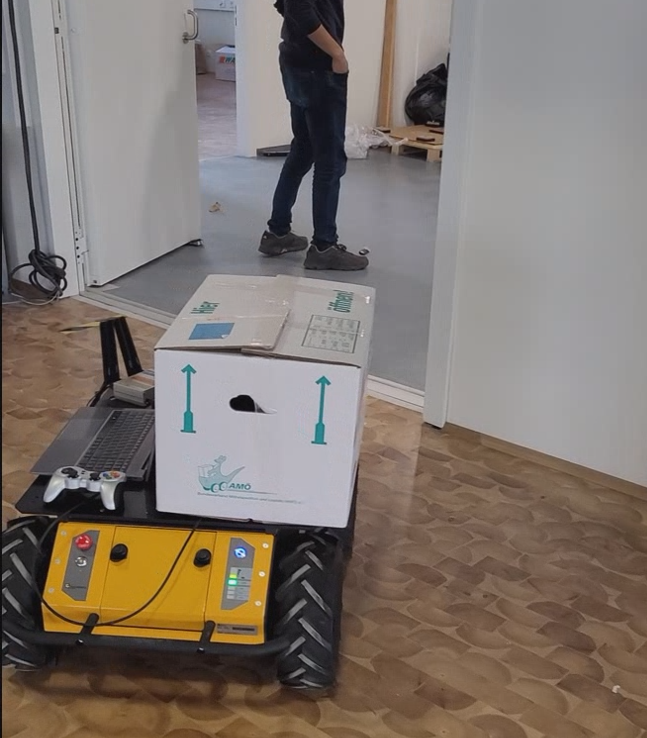
\includegraphics[width=0.9\columnwidth]{pic/movingbox.png}
	\caption{A mobile robot with extended intelligence beyond native, vendor-defined skills. The robot builds and updates a task-grounded, memory-augmented scene graph as a shared mental model for reasoning about dynamic environments, safe navigation, verbally expressed human intent, and real-time spoken feedback, thereby enabling intuitive, programming-free, and inclusive payload transportation.}
	\label{intro}
\end{figure}

Mobile robots are increasingly deployed in everyday societal applications, such as room cleaning and payload transportation, to relieve humans from repetitive and physically demanding tasks \cite{gona2024intelligent,kaigom2023metarobotics,konnecke2024,la2024toward}. Despite this progress, many mobile robots still operate mainly through predefined rules, vendor-defined skills, or fixed task sequences. Such behavior is difficult to scale to human-populated environments, where relevant entities may move, disappear temporarily, reappear in different locations, or become meaningful only through the user’s task intent \cite{kruger2019programming,ajoudani2018progress,beetz2018knowrob,pedersen2016robotics}. As a result, non-expert users often cannot instruct robots naturally to follow, approach, avoid, or reason about objects and people in a way that remains robust under dynamic perception conditions.

Classical mobile robot interaction pipelines typically combine object or person detection with geometric feedback control, for example using proportional-integral-derivative (PID) control to track Cartesian poses estimated from stereo vision \cite{chen2020vision,wu2021person,li2022robust}. While effective for local tracking, these pipelines usually remain reactive: once the target is lost, occluded, ambiguously described, or no longer directly visible, the robot lacks a persistent task-level model for maintaining intent, recovering behavior, or explaining its decisions. Purely descriptive scene understanding also remains insufficient, because a scene description alone does not specify which entities are task-relevant, how they relate to the robot state, or what constraints should guide autonomous action.

This paper proposes an Extended Robot Intelligence (ERI) framework that transforms perception from a sequence of isolated detections into a task-grounded and memory-augmented scene graph (SG). The SG integrates object detections, 3D spatial attributes, robot-state information, user intent, task constraints, confidence values, and interaction history into a persistent semantic representation. Multimodal large language models (MLLMs) \cite{gupta2023vlmaps,huang2023vlfm,konishi2023navgpt} are used not as standalone scene describers, but as reasoning modules operating over structured, task-relevant context. This enables the robot to combine human instruction with constrained autonomous behavior, including ambiguity handling, target persistence, recovery after temporary perception loss, and reduced need for repeated user commands.

The central idea is that mobile robot autonomy should not be limited to either low-level tracking or unrestricted language-driven decision-making. Instead, flexible autonomy can emerge from a shared semantic memory that links what the user means, what the robot perceives, what the robot has recently known, and what actions remain safe and feasible. In this way, the ERI framework supports intuitive, transparent, and programming-free interaction while remaining compatible with resource-constrained mobile robotic platforms.

The main contributions of this work are as follows:

\begin{itemize}
	\item Task-grounded memory-augmented SG:
	We introduce a persistent SG representation that fuses object detections, 3D spatial attributes, robot-state information, task constraints, confidence values, and interaction history. This representation supports temporal continuity, target persistence, and recovery after temporary perception dropouts.
	
	\item Flexible autonomy through structured semantic reasoning:
	We combine deterministic preprocessing, constraint-based filtering, and MLLM reasoning to map natural-language intent onto task-relevant scene entities and feasible robot behavior. This allows the robot to act under human-defined goals while autonomously resolving ambiguity, maintaining context, and adapting to dynamic scenes.
	
	\item Human-centered and resource-efficient deployment:
	We develop a voice-driven interaction pipeline with real-time spoken feedback for intuitive, programming-free robot use. The system reduces repeated user intervention and remains deployable on resource-constrained mobile platforms for inclusive payload transportation and assistive navigation.
	```
	
\end{itemize}

The remainder of this paper is organized as follows. Related work is presented in Fig.~\ref{relatedwork}. The proposed method and its implementation are described in Fig.~\ref{methodology}. The experimental results are presented in Fig.~\ref{sec:experiments}. Finally, Fig.~\ref{conclusion} concludes the paper.



\begin{table*}[!hb]
	\centering
	\caption{Tools and models for 3D SGG, perception, navigation and interfacing in robotics}
	\label{tab:scenegraph_technologies}
	\resizebox{\textwidth}{!}{%
		\begin{tabular}{|l|l|l|l|l|}
			\hline
			\textbf{System/Framework} & \textbf{\begin{tabular}[c]{@{}l@{}}Detection \& Segmentation \\ (Nodes)\end{tabular}} & \textbf{\begin{tabular}[c]{@{}l@{}}Semantic Features \& \\ Embeddings\end{tabular}} & \textbf{\begin{tabular}[c]{@{}l@{}}Relation Inference \& \\ Planning (Edges)\end{tabular}} & \textbf{\begin{tabular}[c]{@{}l@{}}Alternatives \& \\ Additional Models \& \\ Misc. \end{tabular}}  \\ \hline
			\textbf{ConceptGraphs}\cite{conceptgraphs} & SAM & CLIP, Grounding DINO & GPT-4, LLaVA & RAM \\ \hline
			\textbf{3DGraphLLM}\cite{3dgraphllm} & Mask3D, OneFormer3D & DINOv2 (2D), Uni3D (3D) & VL-SAT, CLIP & LLaMA3-8B, Vicuna-1.5 \\ \hline
			\textbf{Graph2Nav}\cite{graph2nav} & PSGFormer, Mask2Former & Panoptic Labels & 2D-PSG Inference, GPT-3.5 & LIO-SAM, Whisper \\ \hline
			\textbf{HOV-SG}\cite{hovsg} & SAM & CLIP & Hierarchical Heuristics & GPT-3.5, GPT-4 \\ \hline
			\textbf{OpenIN}\cite{openin} & CropFormer & SBERT, CLIP & GPT-4o & Tokenize Anything \\ \hline
			\textbf{SG-Nav}\cite{sgnav} & SAM & VLMs, LLMs & LLaMA-7B, GPT-4, LLaVA & Fast Marching Method \\ \hline
			\textbf{Interaction Updates}\cite{interaction} & Existing 3D SG (e.g., Hydra) & Visual Transformer (ViT) & GPT-4, BLIP-2 & DBSCAN (Denoising) \\ \hline
			\textbf{VisionGPT}\cite{visiongpt} & YOLO-World & Proportional 2D Coordinates & GPT-3.5 Turbo, GPT-4 & H-Pattern Splitter \\ \hline
			\textbf{LGX}\cite{lgx} & GLIP, YOLO & BLIP (Captions) & GPT-3 & OWL-ViT, Detectron2 \\ \hline
			\textbf{VLMaps}\cite{gupta2023vlmaps} & LSeg & CLIP & Codex (Code-writing LLM) & RTAB-Map \\ \hline
		\end{tabular}%
	}
\end{table*}


\section{Related Work}\label{relatedwork}
Societal applications typically take place in unstructured environments, such as homes, where multiple objects exhibit spatial, temporal, and contextual dynamics. These changes can arise from uncertain human activities as well as from the appearance and disappearance of entities with specific properties and affordances in the 3D scene \cite{yalcinkaya2024towards}. SGs provide a structured and multimodal representation of the sensed environment, allowing robots to reason about their operational space and generalize appropriate actions. Neural-network-based approaches have therefore been proposed for object detection, scene graph generation (SGG), and interpretation in mobile robotics. The following subsections review relevant methods for SGG and outline their connections to our approach.

\subsection{Scene Graph}\label{scenegraph}

An SG represents a scene in a structured form by encoding objects, their attributes, and relationships. SGG can be derived from images, text, or videos. An SG is a hierarchical graph consisting of nodes $O$ and edges $E$. Nodes represent objects such as humans or items (e.g., bicycle, car), as well as parts of objects (e.g., a person's arm). Each node may include attributes describing the object's state, such as color, size, or pose. Edges often represent relationships between object pairs, describing actions (e.g., man holds cup) or spatial relations (e.g., man stands in front of bench). These relationships are typically expressed as triples 
$\langle \text{subject} - \text{predicate} - \text{object} \rangle$ \cite{li2024scene}.
\subsection{Tools for Scene Graph Generation}
\noindent Various models and technologies are used for SGG across robotics, computer vision, autonomous navigation, and human-machine interaction (see Table~\ref{tab:scenegraph_technologies}). Recent advances in Foundation Models have shifted the field from class-limited object recognition toward universal segmentation models (e.g., Segment Anything Model (SAM/SAM2)~\cite{jiaxing2025sam2}) and open-vocabulary encoders such as Contrastive Language–Image Pretraining (CLIP)~\cite{chen2024clip}, which provide pixel-accurate masks and semantic embeddings. These capabilities allow modern MLLMs and Vision-Language Models (VLMs) to recognize not only object classes but also semantic states and complex relationships. Frameworks such as ConceptGraphs~\cite{gu2024conceptgraphs} and 3DGraphLLM~\cite{zemskova20253dgraphllm} leverage this information to construct SGs interpretable for LLMs while grounding objects in 3D space using geometric data from sensors such as Light Detection and Ranging (LiDAR) or depth cameras. 

Other approaches, including VLMaps~\cite{huang2023visual} and Graph2Nav~\cite{shan2025graph2nav}, translate these spatial relations directly into navigation commands. Many existing frameworks require prior mapping or 3D reconstruction \cite{3dgraphllm,hovsg,openin,interaction}, while others construct maps online in previously unknown environments \cite{conceptgraphs,graph2nav,sgnav,lgx,gupta2023vlmaps}. However, such approaches typically depend on powerful hardware, multiple sensors, and extensive preprocessing, often involving LiDAR or depth-based scanning of entire environments. The resulting maps are then enriched with semantic descriptions, for instance through MLLMs, enabling tasks such as visual question answering about specific objects. In contrast, our approach aims to be resource-efficient and cost-effective. It generates a SG directly from the current image only when needed (e.g., to describe the scene), avoiding time-consuming mapping and enabling dynamic operation.

\subsection{Layered Architecture for Scene Graph}

Mobile robots can reason over contextualized and structured information to plan and achieve goals. Recently, SGs have been adapted for mobile robotics, and multiple abstraction layers of real-world scenes have been introduced for this purpose. These include the spatial layer, which represents locations within the scene; the semantic layer, which captures the meaning of entities, including their states, affordances, predicates, and other attributes; the topological layer, which represents connectivity between locations; and the task-related layer, which encodes robot goals \cite{rana2023sayplan,im2024egtr}. Entities  in the scene populate these layers, which differ in several respects. One such distinction is the update rate of entity attributes \cite{rana2023sayplan,im2024egtr}. For example, the robot initial and final positions may be known in advance and can therefore be treated as fixed, whereas task completion may be required within a short time window, prompting the robot to execute motions more quickly. In contrast, in entity-following applications, the robot desired position changes over time, indicating a dependence of the scene perception on the task and robot dynamics  often omitted.


\begin{figure}[!t]
	\centering
	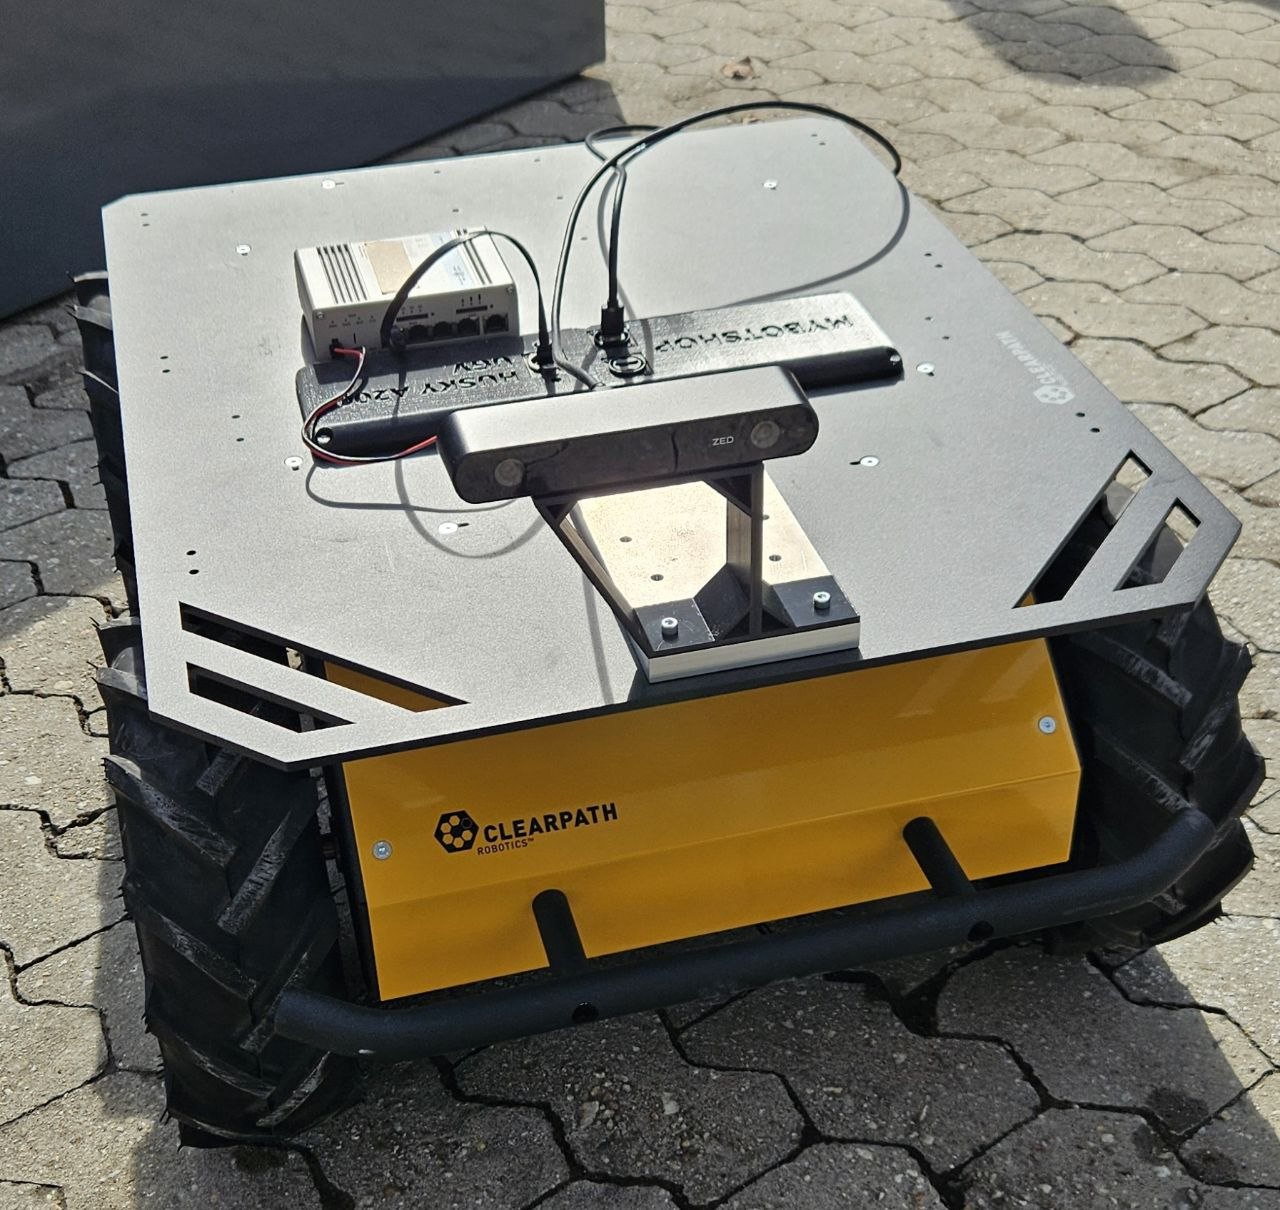
\includegraphics[width=3.2in]{images/husky_zed.jpg}
	\caption{Husky Robot as a mounting platform for the ZED 2i camera.}
	\label{husky_robot}
\end{figure}

In this work, to ensure task relevance and physical feasibility, we employ a hybrid rule- and constraint-based filtering layer coupled with MLLM reasoning. Rule-based components encode spatial, semantic, and task-specific knowledge (e.g., distance thresholds, motion classification, and target selection), while constraint-based components enforce feasibility conditions such as safety, kinematics, and perception confidence. The resulting structured and task-grounded representation is used to construct a prompt for the MLLM, which performs high-level semantic reasoning. This allows the model to infer task-relevant relationships, resolve ambiguities, and generate human-interpretable scene descriptions. By combining rule-based pre-processing, constraint enforcement, and MLLM reasoning, the system produces a dynamic SG that is both semantically meaningful and operationally valid for real-world robotic tasks. Unlike purely rule-based SGs, our hybrid approach enriches the SG with conversation history and task-related experiences, resulting in a memory-augmented representation. Using the profile history to anticipate object affordance and actions enhances  user experience.

\begin{comment}

  \begin{table}[!t]
	\centering
	\caption{Classification of  Algorithms and Inference Concepts for SGG.}
	\label{tab:features}
	\begin{tabular}{|c|c|c|c|}
		\hline
		\textbf{Source} & \textbf{Feature representation} & \textbf{Method for relation inference} \\
		\hline \hline
		\cite{kim2025semantic,su2024adopting} & Box-based &  MPNN, CNN    \\
		\hline
		\cite{im2024egtr,hao2025bctr} & Query-based &  Attention mechanism  \\
		\hline
		\cite{liu2021fully,newell2017pixels} & Point-based &  CNN \\
		\hline
	\end{tabular}
\end{table}

	Inhalt...
\end{comment}

%\subsection{Algorithms for the generation of scene graphs}
%Three main classes of feature representation and  relation inference have emerged in SGG (see Fig.~\ref{tab:features}). Semantic SGG has recently shifted the focus from object- to relation-centric to handle multi-object relationships in real scenes \cite{kim2025semantic}. The approach combines object detection based on a fast Region-based Convolutional Neural Network (R-CNN), an edge-dual scene graph, and an object-relation-centric Message Passing Neural Network (MPNN). The MPNN aggregates information from neighboring entities to learn object- and relation-centric features, enabling iterative updates of entity representations and producing a feature vector for the entire graph \cite{kim2025semantic,su2024adopting}. Recent SGG approaches also exploit attention mechanisms by connecting objects with significant attention weights derived from the self-attention layers of a pre-trained DEtection TRansformer (DETR) \cite{im2024egtr}. A third strategy is Convolutional Scene Graph Generation (CSGG), where objects are encoded as bounding-box center points and relationships are represented as 2D vector fields pointing from subject to object \cite{liu2021fully}. Key characteristics of these approaches are summarized in \cite{liu2024repsgg} and reported in Fig.~\ref{tab:features}.  We use a box-based approach (YOLO (You Only Look Once), CNN) and extend it with an MLLM to determine relations between objects. To this end, we combine a deterministic preprocessing (see Fig. \ref{transformation_template}), natural language, and logical inference to enable societal robot reasoning.


%\subsection{Tools for the genereration of scene graphs}

%Different tools have been developed to perform the intermediate operations required for SGG from sensed data. An overview of these tools is presented in Fig.~\ref{tab:scenegraph_technologies}. For example, YOLO and SAM (Segment Anything Model) play key roles in object detection and segmentation tasks. SAM is a general-purpose model capable of performing pixel-level segmentation, whereas YOLO primarily provides bounding-box detection. YOLO is specifically optimized for low latency, making it suitable for real-time scenarios in dynamic, human-centered environments where rapid collision avoidance is critical. This enables faster collision handling while the system follows human motion paths within our framework. CLIP is widely used for extracting semantic features due to its open-vocabulary capabilities. It supports multimodal classification at both the pixel and bounding-box levels. The shared semantic embedding space provided by CLIP enables a seamless transition from image-based perception to language-driven understanding, for example through GPT-based prompting.


\subsection{Operationalization  of Scene Graphs}
SGs have been used in  societal applications, such as finding seating in indoor environments \cite{ravichandran2025safety}, assisting with cooking \cite{kwon2025large}, and supporting city-scale inspection missions \cite{viswanathan2024xflie,amiri2022reasoning}. However, most SGs are constructed from single images, whereas human activities typically span longer time horizons. To address long-term goals, \cite{ravichandran2025safety} federates local SGs from successive images into a global SG. In contrast, our approach leverages an MLLM that exploits reasoning history and generalization capabilities for long-term reasoning. Similar contextual grounding is explored in \cite{kwon2025large} using the generative capabilities of an LLM. We extend this scene-centered contextualization by considering internal robotic processes, including sensed kinematic behavior, motion dynamics, and predicted energy consumption. Our framework thereby unifies scene awareness,  motion planning, and feasibility assessment. By leveraging AI-based SGs and MLLMs, the robot achieves enhanced visual and semantic awareness of the environment, including areas not directly perceived by human teammates. We define this novel capability, which bridges scene-level \textit{perception} and system-level introspection through MLLM reasoning, as \textit{pAIrSEEption}. This capability enables the robot to assist and guide humans in real-world applications via natural spoken language. Its key components are illustrated in~Fig.~\ref{overview_framework}.

\begin{figure}[!t]
	\centering
	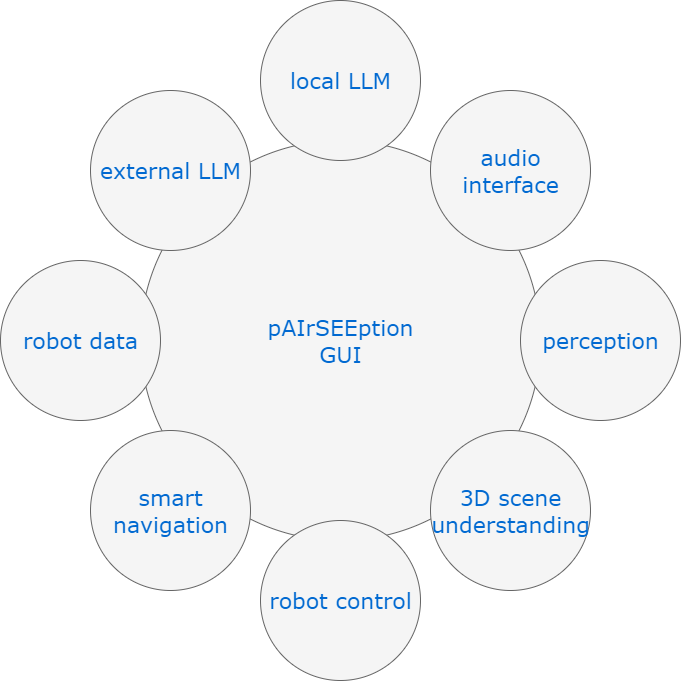
\includegraphics[width=2.4in]{images/overview_eng.png}
	\caption{Features and components of the pAIrSEEption functionality.}
	\label{overview_framework}
\end{figure}

\section{Methodology}\label{methodology}
%This section presents  developed methods and their implementation. 

\subsection{Overview of Features and Components}

\textit{pAIrSEEption} provides a multi-modal access to the  perception, reasoning, and introspection of the robotic system, aligned with human perceptual modalities such as vision, hearing, and speech through AI-driven integration. At its core, it leverages a memory-augmented SG that integrates structured environmental and robot-state information with past interactions and task experience. This enables natural, context-aware human-robot teaming for assistance and guidance without requiring users to write code. Live audio feedback, visual awareness of the environment, and monitoring of the robot’s intentions and predicted performance can be dynamically customized through the responsive GUI in Fig.~\ref{framework_architecture}. By grounding interactions in the SG’s memory via MLLM reasoning, \textit{pAIrSEEption}  provides continuity, adaptability, and robustness to perception uncertainty and evolving task contexts.

The GUI is platform-independent. It can be deployed on different devices, such as the  Jetson AGX Orin (32\,GB) edge platform onboard or a standard laptop with  integrated Nvidia GPU. A ZED~2i stereo camera is connected to these devices for perception. Its wide $110^\circ\text{(H)}\times70^\circ \text{(V)}\times120^\circ \text{(D)}$  field of view is used to capture context-relevant details beyond the user’s line of sight, while providing robust performance under varying lighting and texture conditions. The PID-controlled mobile Husky UGV robot~\cite{husky} is the mounting platform for  hardware components (see Fig.~\ref{husky_robot}). The GUI serves as  visualization and control center of the system, where all  data streams are integrated. The interface displays the following information:







\begin{itemize}
	\item A live annotated stereo-camera video stream from the perception pipeline. 
	\item System performance statistics, such as frames per second (FPS) and utilization of  CPU, GPU, VRAM, and RAM.
	\item Status and system messages indicating active or inactive processes.
	\item Transcribed user voice commands for quality check.
	\item Scene descriptions and conversational responses generated by the LLM based on object data and current images.
	\item Navigation control for selecting detected objects to follow or approach, simplifying target selection even remotely.
	\item Internal robot diagnostics (e.g., motor temperatures) queried via voice commands and displayed in the GUI.
\end{itemize}

Displayed data, along with user voice inputs, can be stored locally in common file formats through the GUI. This enables dataset collection for potential future fine-tuning or training of the YOLO (You Only Look Once) and MLLM models.




\begin{figure*}[!t]
	\centering
	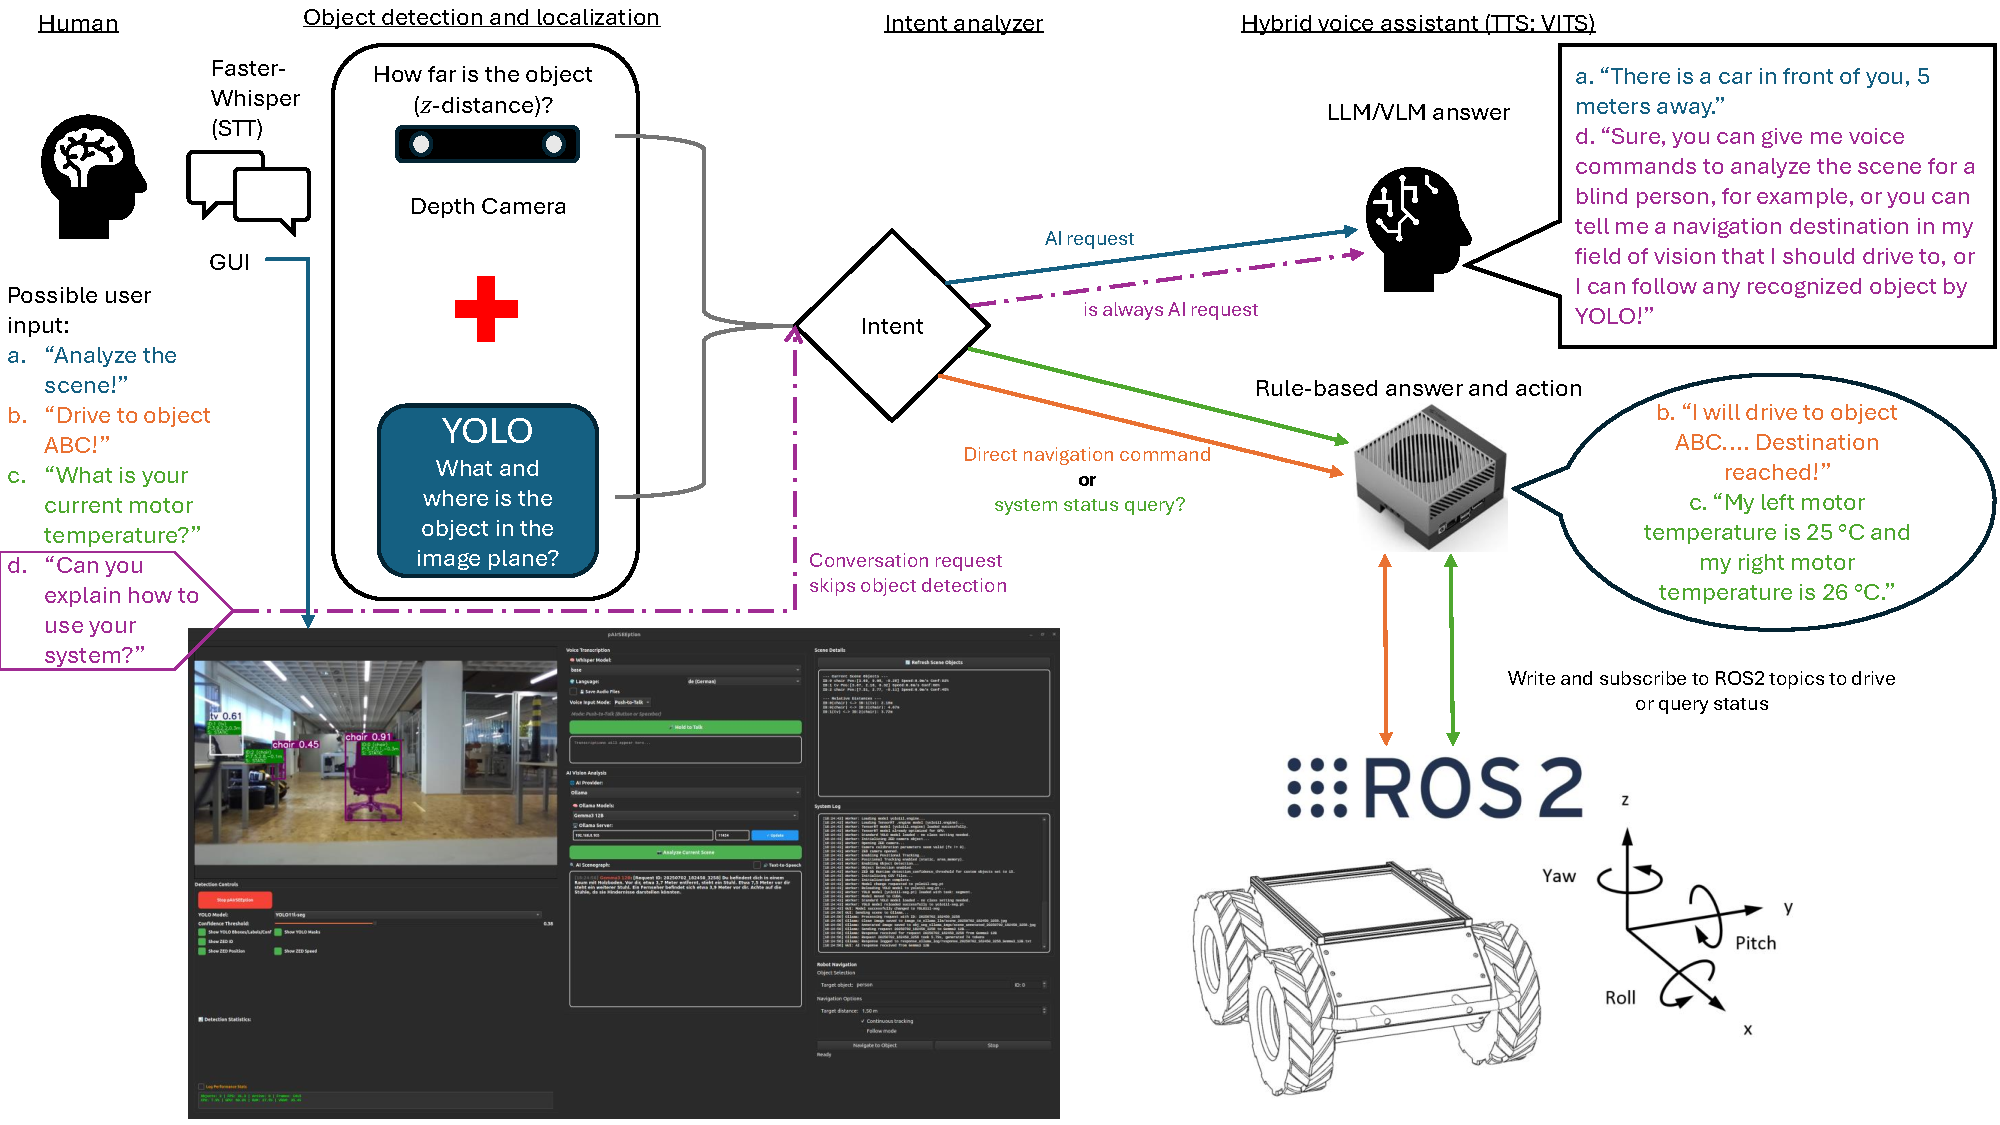
\includegraphics[width=\textwidth]{images/framework_architecture.pdf}
	\caption{System components and data processing pipeline (reading from left to right).}
	\label{framework_architecture}
\end{figure*}

\subsection{Data Processing Pipeline}

The interface provides multiple versions and sizes of YOLO and YOLOE (open-vocabulary) models for object detection and segmentation, as well as MLLMs for scene interpretation. These options can be extended as needed. The GUI also allows configuration of YOLO parameters, including the display of bounding boxes, classification labels, and confidence values. A confidence slider enables filtering of detections below a selected threshold.

The data flow throughout the system is organized into five layers (see Fig.~\ref{framework_architecture}, reading from left to right):


\begin{enumerate}
	\item Voice (speech-to-text, STT) or text input via the GUI (e.g., scene description, navigation goal, robot status, or casual conversation).
	\item Object detection with distance estimation. This step is skipped when a purely conversational interaction with the MLLM is requested.
	\item Preprocessing through a rule-based intent analyzer that determines the requested task. Although this component could be replaced by a lightweight LLM orchestrator, the rule-based approach offers lower latency and greater resource efficiency, which is important in time-critical scenarios.
	\item Hybrid response generation via either the MLLM or predefined rule-based messages. All responses are communicated through the text-to-speech (TTS) system. Scene descriptions and conversations are handled by the MLLM, while robot status queries and navigation commands (e.g., following or approaching an object) are processed through rule-based logic.
	\item When navigation or system status is requested, the system publishes or subscribes to ROS2 topics to control the robot or retrieve status information.
\end{enumerate}


\subsection{Task Grounding}
\label{taskgrounding}

Task grounding in \textit{pAIrSEEption} connects human intent, visual perception, and executable robot behavior. The system grounds user commands in detected objects by combining YOLO-based object detection, ZED~2i depth measurements, speech-based intent extraction, and structured prompt generation for the MLLM. The resulting grounding interface converts noisy human input and frame-wise detections into action-constrained, prompt-ready object representations. Rather than querying the MLLM with raw visual input alone, the proposed grounding layer constrains multimodal reasoning through robot-actionable object states, including class labels, assigned identifiers, 3D positions, motion states, and task-specific constraints.

YOLO-based object detection serves three purposes in the system. First, YOLO provides real-time 2D detections that are fused with ZED~2i depth measurements via the ZED SDK to estimate spatial object information, such as object distance and 3D position; see Fig.~\ref{framework_architecture}. These data are transformed into a structured textual representation, as illustrated in Fig.~\ref{transformation_template}, and passed to the MLLM as part of the grounded input prompt. Second, although modern MLLMs and VLMs can generate 2D bounding boxes, YOLO is used as a lightweight preliminary detection layer to reduce the computational load on the MLLM and minimize inference latency. Third, the detections provide the perceptual basis for navigation and object-following. For this purpose, object-camera distances and pairwise inter-object distances are computed using the 3D Euclidean metric. The target object is selected through its object class and an assigned object identifier, which is maintained by the perception and memory pipeline. The target can be specified either via the graphical interface or by voice input.

Voice-based task grounding is achieved through semantic task mapping. The system translates unstructured and potentially noisy human speech into structured machine commands. Voice transcription is performed using faster-whisper \cite{fasterwhisper}. The transcribed text is then processed in two stages. First, an integrated speech intent parser applies rule-based pattern matching using regular expressions (regex), as depicted in Fig.~\ref{fig:regex_pipeline}. Second, fuzzy string matching is used as a fallback mechanism to correct common transcription errors and map spoken requests to robot commands such as ``navigate'' or ``follow'' when the regex rules do not recognize the intent. Spoken object names are mapped to valid YOLO classes, ensuring that the user's verbal intent remains grounded in the robot's perceptual capabilities.

\begin{figure*}[t]
	\centering
	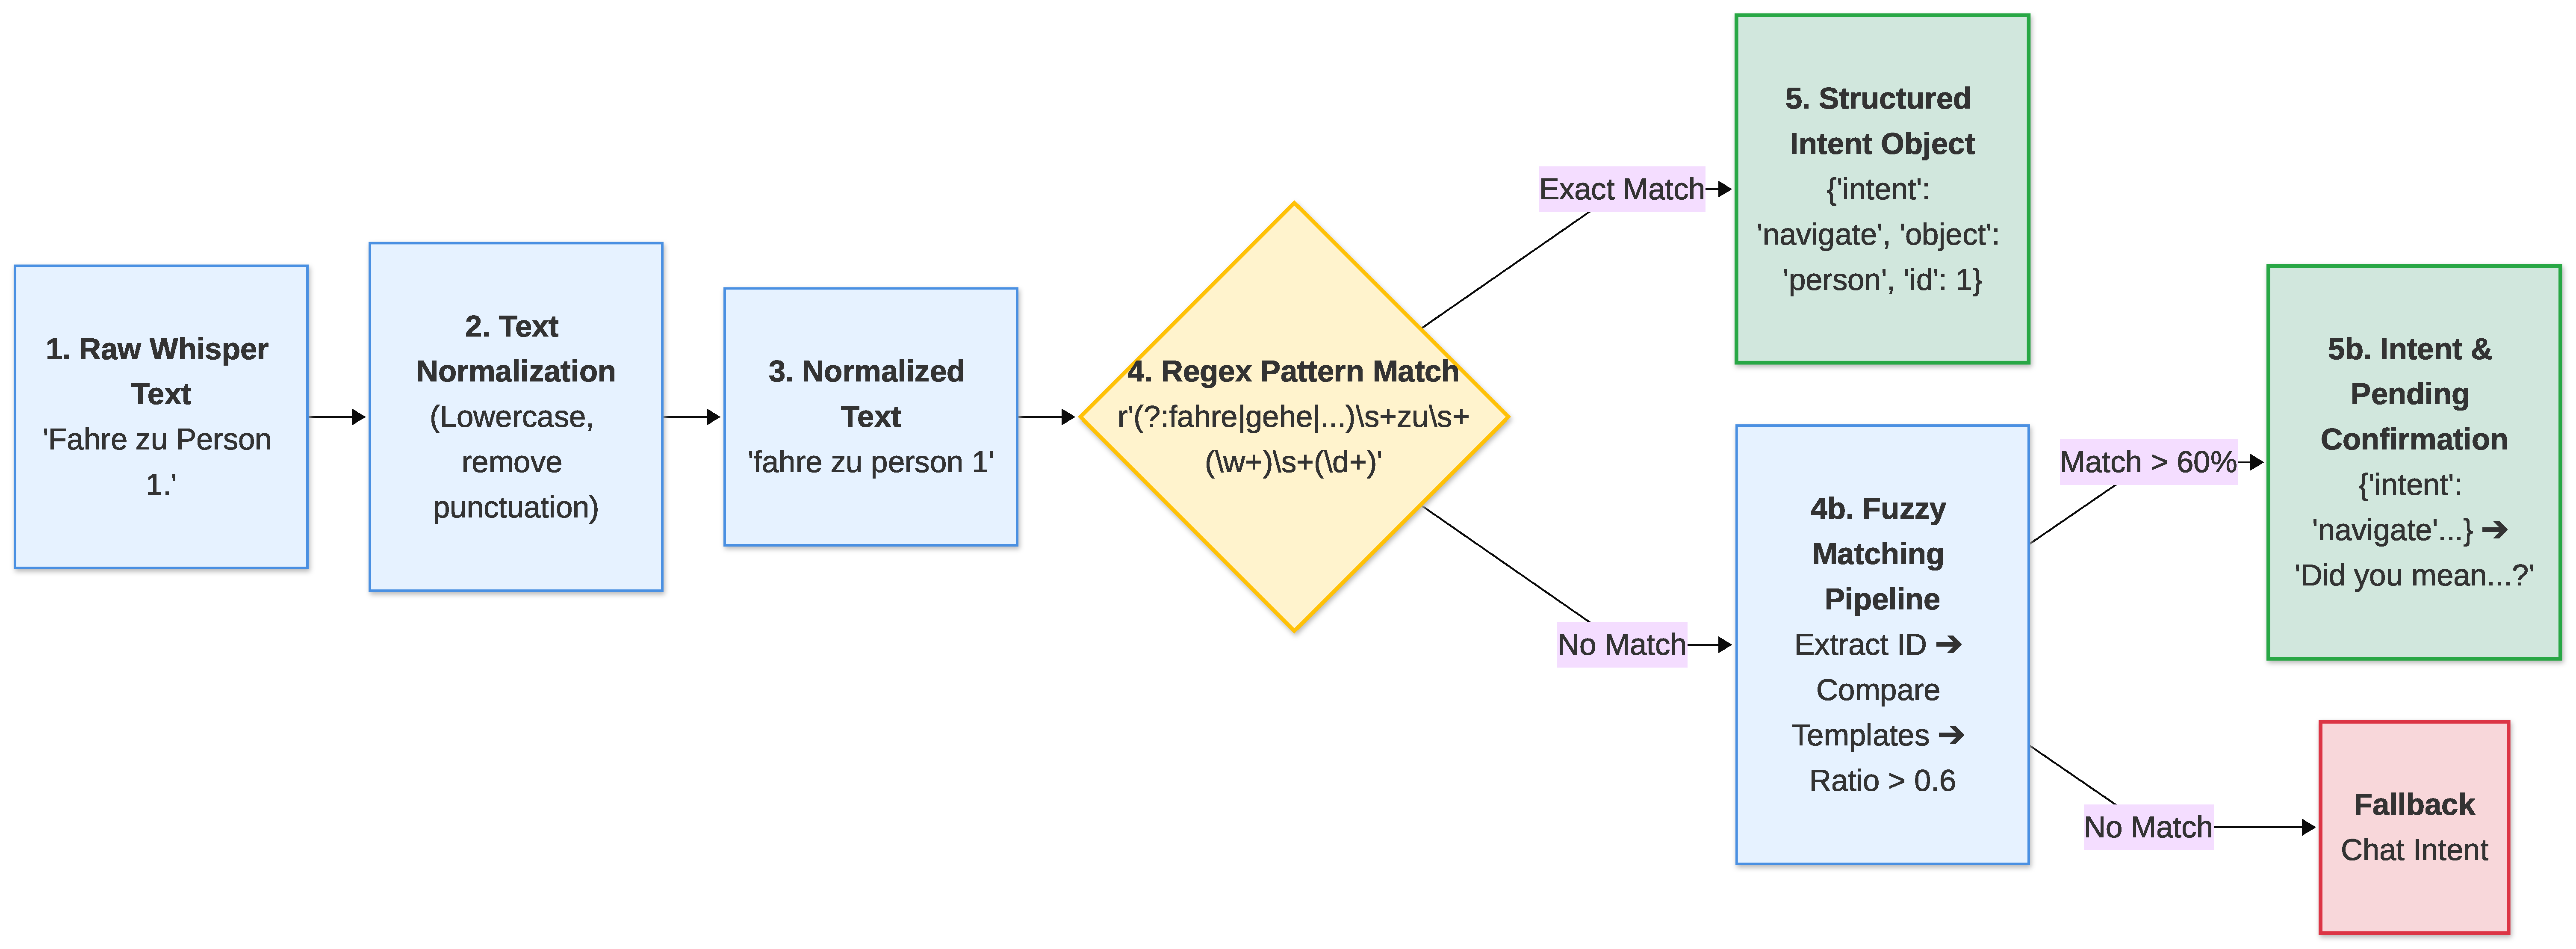
\includegraphics[width=1.0\textwidth]{images/regexfuzzymatching.pdf}
	\caption{After text normalization and regular expression (Regex) matching, a fuzzy-matching pipeline resolves navigation intents from noisy transcriptions. The depicted examples are in German as processed by the system's voice interface.}
	\label{fig:regex_pipeline}
\end{figure*}




In \textit{pAIrSEEption}, a detected object is represented by its semantic class and a set of spatial and dynamic attributes. For example, a detected person can be represented as
\begin{equation}
	\begin{aligned}
		o_1 = \Bigl(\text{person},
		\left\{
		\begin{aligned}
			& \text{ID} = 1, \\
			& \text{confidence value} = 0.95, \\
			& \text{3D position} = (x, y, z), \\
			& \text{3D velocity} = (v_x, v_y, v_z), \\
			& \text{motion state} = \text{static}
		\end{aligned}
		\right\}
		\Bigr).
	\end{aligned}
	\label{eq:o1}
\end{equation}

The object \(o_1\) is therefore described by an identifier, a confidence score, a 3D position, a 3D velocity, and a motion-state classification. The spatial quantities are expressed in the depth-camera reference frame, such that the estimated position \((x,y,z)\) and velocity \((v_x,v_y,v_z)\) are defined relative to the camera. The motion state is classified as \textit{static} when the velocity magnitude remains below a predefined threshold, i.e., \(\lVert v \rVert < \epsilon_v\). This threshold-based formulation avoids treating small measurement noise as object motion.

The structured object data are then mapped to task-relevant candidates by linking the parsed user command to object classes, identifiers, spatial relations, and motion states. Before the grounded object data are passed to the MLLM, rule-based filtering applies physical and kinematic constraints. For example, the operator can specify the distance that should be maintained to a target object or stop the robot in critical situations using a voice command. This step ensures that the MLLM does not reason over raw detections alone, but over perception data that are already constrained by the robot's executable action space.




To reduce computational load, the MLLM processes a single image together with the structured object description. Since object motion cannot be inferred reliably from a single image alone, the object description additionally includes velocity and motion-state information derived from the perception pipeline. This design allows the MLLM to generate scene descriptions that account for both spatial layout and object motion while avoiding repeated multi-frame requests. The following prompt is used to instruct the MLLM to analyze the image and the associated object data for safe navigation of visually impaired users:

\noindent
\begin{center}
	\fcolorbox{black}{black!5}{%
		\begin{minipage}{0.92\columnwidth}
			\setlength{\parskip}{0.5em}
			\ttfamily
			Describe the image briefly and precisely using the object data provided.
			
			\{object\_description\}
			
			Describe what can be seen in the image,
			where important objects are located,
			and provide information about possible obstacles.
		\end{minipage}%
	}
\end{center}


The variable \textit{object\_description} contains the structured object data generated during preprocessing. Initially, a deterministic template was used to convert raw detections into concise textual bullet points. Fig.~\ref{transformation_template} illustrates this transformation. By combining image input with structured object data, the MLLM generates a human-readable description of the 3D scene that is grounded in the robot's perception pipeline rather than relying on image-level reasoning alone. This grounding strategy transforms MLLM input from an unconstrained image-captioning problem into a robot-actionable scene representation in which object references, spatial relations, motion states, and user commands are explicitly aligned before inference.

\subsection{Memory Augmentation}
\label{memoryaugmentation}

\begin{figure}[!b]
	\centering
	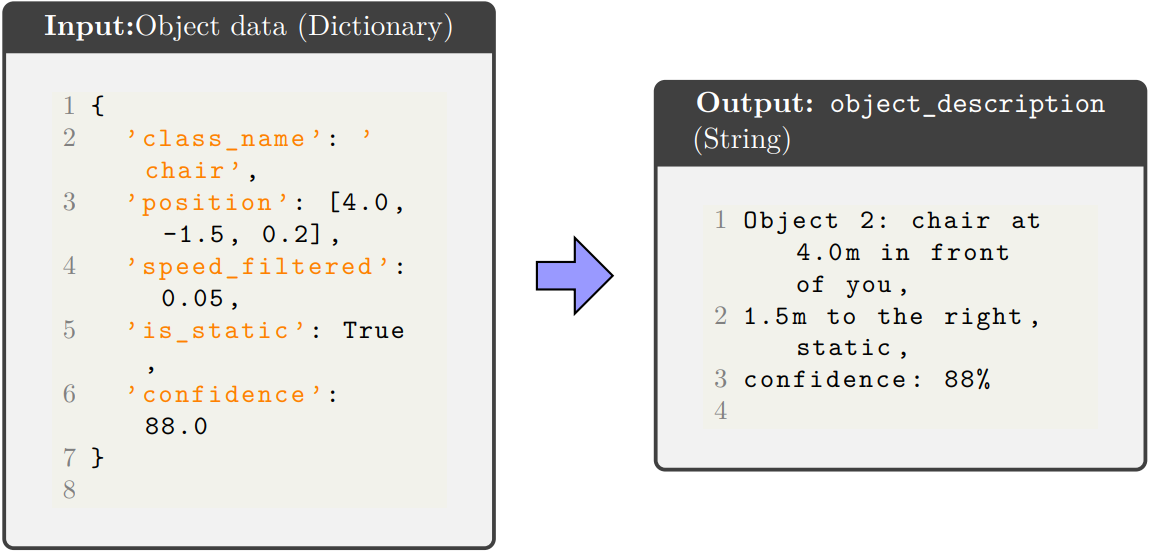
\includegraphics[width=\columnwidth]{images/transformation_template.png}
	\caption{Data preprocessing: transformation of object data into a readable description for prompt input.}
	\label{transformation_template}
\end{figure}


Frame-wise perception provides only a transient representation of the current camera view. This is insufficient for interactive robot navigation, where objects may be temporarily occluded, leave the field of view, reappear later, or become ambiguous when several instances of the same class are present. To address this limitation, \textit{pAIrSEEption} constructs a memory-augmented scene graph (SG) that combines structured perception outputs, robot-state information, and MLLM-generated semantic and task-grounded attributes.

Each detected object is represented by geometric, semantic, and interaction-related attributes. Geometric attributes describe the object position, camera-relative distance, inter-object distance, and motion state. Semantic attributes specify the object class, confidence score, visibility status, and MLLM-generated scene role. Interaction-related attributes encode whether an object is currently relevant for navigation, following, obstacle avoidance, or user clarification. The resulting SG is maintained as an in-memory scene representation during runtime, allowing fast updates of object states, temporal descriptors, and task-relevance indicators. For transparent inspection, reproducibility, and lightweight persistence, selected memory states are serialized into structured CSV and text-based records. Thus, CSV files are not used as the primary representation for reasoning, but as an export and persistence mechanism for a backend-independent memory abstraction. This design allows the task-grounding pipeline to be extended toward graph databases, RDF/OWL representations, or other ontology-based memory structures without modifying the interaction logic.



The memory architecture combines short-term and long-term memory. Short-term memory stores the most recent reliable state of each object, such as its identifier, spatial coordinates, confidence score, visibility status, and task role. This information is reused when an object temporarily leaves and later re-enters the field of view; see Fig.~\ref{renentrance}. If an object is no longer detected because of occlusion, viewpoint change, or a temporary drop in detection confidence, the memory-augmented SG retains the corresponding node within a finite temporal validity window instead of removing it immediately. During this interval, the object is marked as temporarily unobserved, while its last reliable position, identifier, task role, and confidence history remain available for reasoning. This hysteresis-like retention mechanism improves temporal consistency, reduces sensitivity to short perception dropouts, and prevents premature target switching during navigation or object-following.

\begin{figure*}[t!]
	\centering
	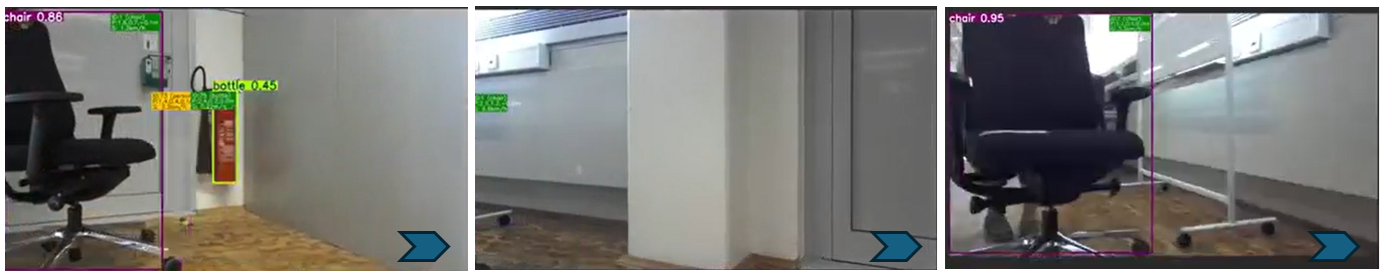
\includegraphics[width=2\columnwidth]{images/reentrance.png}
	\caption{Memory recall evaluation: User queries a chair that has left the scene, and the SG correctly retrieves its past and current attributes from memory.}
	\label{renentrance} %\label{SGmemory}
\end{figure*}

Long-term memory provides a compact historical context layer that converts previous observations into task-relevant descriptors rather than replaying raw logs. The system processes object histories, tracking information, and distance metrics to estimate how frequently an object has been observed, how stable its detections are, whether its spatial relation to the robot has changed, and whether recurring interaction patterns exist. These statistics are summarized into memory descriptors, such as observation frequency, average confidence, last known position, spatial persistence, and recent interaction history. By passing these compact descriptors to the MLLM, the system preserves temporal cues needed for scene interpretation, object-reference disambiguation, and interaction-level decision support while keeping the prompt within the context-window constraints.

Memory augmentation is particularly important when user commands are underspecified relative to the perceived scene. Ambiguity arises when a spoken or GUI-based request refers to an object class, such as `car'' or `person'', but the current SG contains multiple candidate nodes that satisfy this reference. In this case, a frame-wise perception system can detect the candidates but cannot determine which instance the user intends to address. In \textit{pAIrSEEption}, the navigation agent first maps the user request to a semantic object class and retrieves all matching nodes from the memory-augmented SG. Candidate objects are then compared using their identifiers, spatial relations to the robot and user, visibility state, confidence history, and recent interaction context. If this comparison does not yield a unique target, the system formulates an explicit clarification question. For example, if two cars are detected, the system may ask: ``I see car 1 on the left and car 5 farther ahead. Which one do you mean?'' The operator can resolve the ambiguity through voice input or the graphical interface. The response is then mapped back to the selected SG node, allowing the robot to continue with a grounded command rather than executing an underspecified action. This closes the loop between perception, memory, language-based clarification, and executable robot behavior, extending the SG from a descriptive representation to an interaction-level grounding mechanism.

The generated scene interpretation is displayed in the GUI output window and can optionally be played back through the TTS system. This output is not generated from the image alone, but from a temporally grounded representation that combines perception-derived geometry, memory-based object persistence, and MLLM-based semantic interpretation. As a result, the interface can report not only what is currently visible, but also which objects are persistent, temporarily unobserved, ambiguous, or relevant to the current task. This supports assistive navigation by providing blind or visually impaired users with scene descriptions that remain consistent across short perception gaps and include clarification when object references are ambiguous. The same mechanism can support human-robot collaboration in semi-structured environments by exposing the robot's scene representation, task interpretation, and uncertainty handling in an interpretable form.

\subsection{Memory-Augmented Task-Grounded Autonomy}
\label{memory_augmented_task_grounding}

Task grounding maps user commands to object classes, assigned identifiers, spatial relations, motion states, and executable constraints. Memory augmentation extends this mapping across time by preserving object states during short perception gaps, summarizing previous observations, and supporting disambiguation when multiple candidate objects satisfy the same user reference. The same memory layer can also support autonomous subgoal selection by providing temporally persistent information about last known object positions, spatial persistence, confidence stability, and recent interaction context. Thus, memory does not only stabilize scene interpretation, but also enables the robot to choose intermediate action references that remain transparent to the human while not requiring explicit operator specification.

The proposed concept of memory-augmented task-grounded autonomy frames autonomy not as a fixed level, but as an adaptive position along an autonomy continuum. The autonomy continuum describes how control is allocated between the human operator and the robot. In \textit{pAIrSEEption}, this continuum ranges from memory-enabled autonomous subtask execution, through task-grounded shared autonomy, to supervised interaction with explicit human clarification. At the autonomous end, the robot can use memory-augmented scene context to make intermediate decisions, such as selecting an intermediate location, maintaining a target reference across short perception gaps, or moving toward a previously observed object region without requiring continuous human intervention. At the shared-autonomy level, the user specifies the task or target class, while the robot grounds the command in object states, spatial relations, and executable constraints. When grounding remains ambiguous or uncertain, the system shifts toward supervised interaction by requesting clarification.

This coupling enables elastic autonomy, understood here as the ability of the robot to move along the autonomy continuum according to grounding reliability and task requirements. When the task goal and relevant scene state are sufficiently grounded, the robot can autonomously execute intermediate steps using memory-augmented SG nodes as action references. When the user specifies a task but leaves the target reference underspecified, the system operates in a task-grounded shared-autonomy mode. For example, a command such as ``drive to the car'' is first mapped to the semantic class \textit{car}. The system then retrieves candidate object nodes from the memory-augmented SG and evaluates them using current visibility, assigned identifiers, spatial relations, confidence history, and recent interaction context. If a unique target can be inferred, the corresponding SG node becomes the executable task reference. If several candidates remain plausible, as depicted in Fig.~\ref{scenememory}, the system shifts toward supervised interaction and formulates a clarification question ``I see car 1 and 5. Which one do you mean?'' before executing the command.

The resulting autonomy is therefore not based on unrestricted MLLM reasoning or unbounded command interpretation. Instead, it is constrained by robot-actionable object states and memory descriptors that make the system's decisions traceable to perception and interaction history. Memory-augmented task grounding acts as the regulating mechanism that determines whether the robot can proceed autonomously, operate in shared autonomy, or request human supervision. In this way, the SG is extended from a descriptive scene representation to an autonomy mechanism for temporally consistent, disambiguated, and human-aligned robot behavior.

\subsection{MLLM Deployment Architecture}
\label{mllm_deployment_architecture}

The system supports different MLLM deployment modes and distinguishes between locally hosted and cloud-based models. Local models are executed through an Ollama-based backend and can run on consumer PCs or edge devices, such as the Jetson Orin, depending on model size, quantization level, and available hardware resources. In the current implementation, Gemma~3 and Qwen~2.5~VL are considered as representative local multimodal models. Gemma~3 supports multimodal input with a large context window and improved attention to small visual details, whereas Qwen~2.5~VL is particularly suitable for image captioning and text-rich visual scenes. Both models support multilingual interaction and offer multiple quantization options~\cite{gemma3,qwen25vl}.

Running models locally provides advantages such as data privacy, version control, and offline operation. However, local inference requires suitable computing hardware and may limit the model size that can be used in real time. As an alternative, cloud-hosted models can be accessed through the OpenRouter API, which provides access to models from different providers. This deployment mode reduces local hardware requirements because inference is executed on external servers. At the same time, it introduces dependencies on network availability, server-side latency, data-transfer constraints, and request-based cost.

To support both deployment modes, the system implements a client-server architecture based on a REST API. The graphical user interface acts as the client and transmits the current image together with the structured object description generated by the task-grounding pipeline. The MLLM server receives this multimodal prompt, performs inference using either a local or cloud-based model, and returns a textual scene interpretation to the GUI. This separation allows the perception and interaction modules to remain independent of the selected model backend.

The server processes a single image together with structured object data, including object class, identifier, 3D position, distance, and motion-state information. This design is important because motion cannot be inferred reliably from a single image alone. By adding velocity and motion-state information from the perception pipeline, the MLLM can reason about whether relevant objects are moving or stationary without requiring multi-frame visual input. Processing single images instead of image sequences reduces computational load and avoids excessive requests to the MLLM, especially when cloud-based inference is used.

This architecture therefore provides a flexible interface between embodied perception and multimodal language reasoning. Local deployment supports privacy-sensitive and offline scenarios, while cloud-based deployment enables access to larger models when network access and request latency are acceptable. In both cases, the MLLM receives perception-grounded scene information rather than raw image input alone.


\begin{figure}[t]
	\centering
	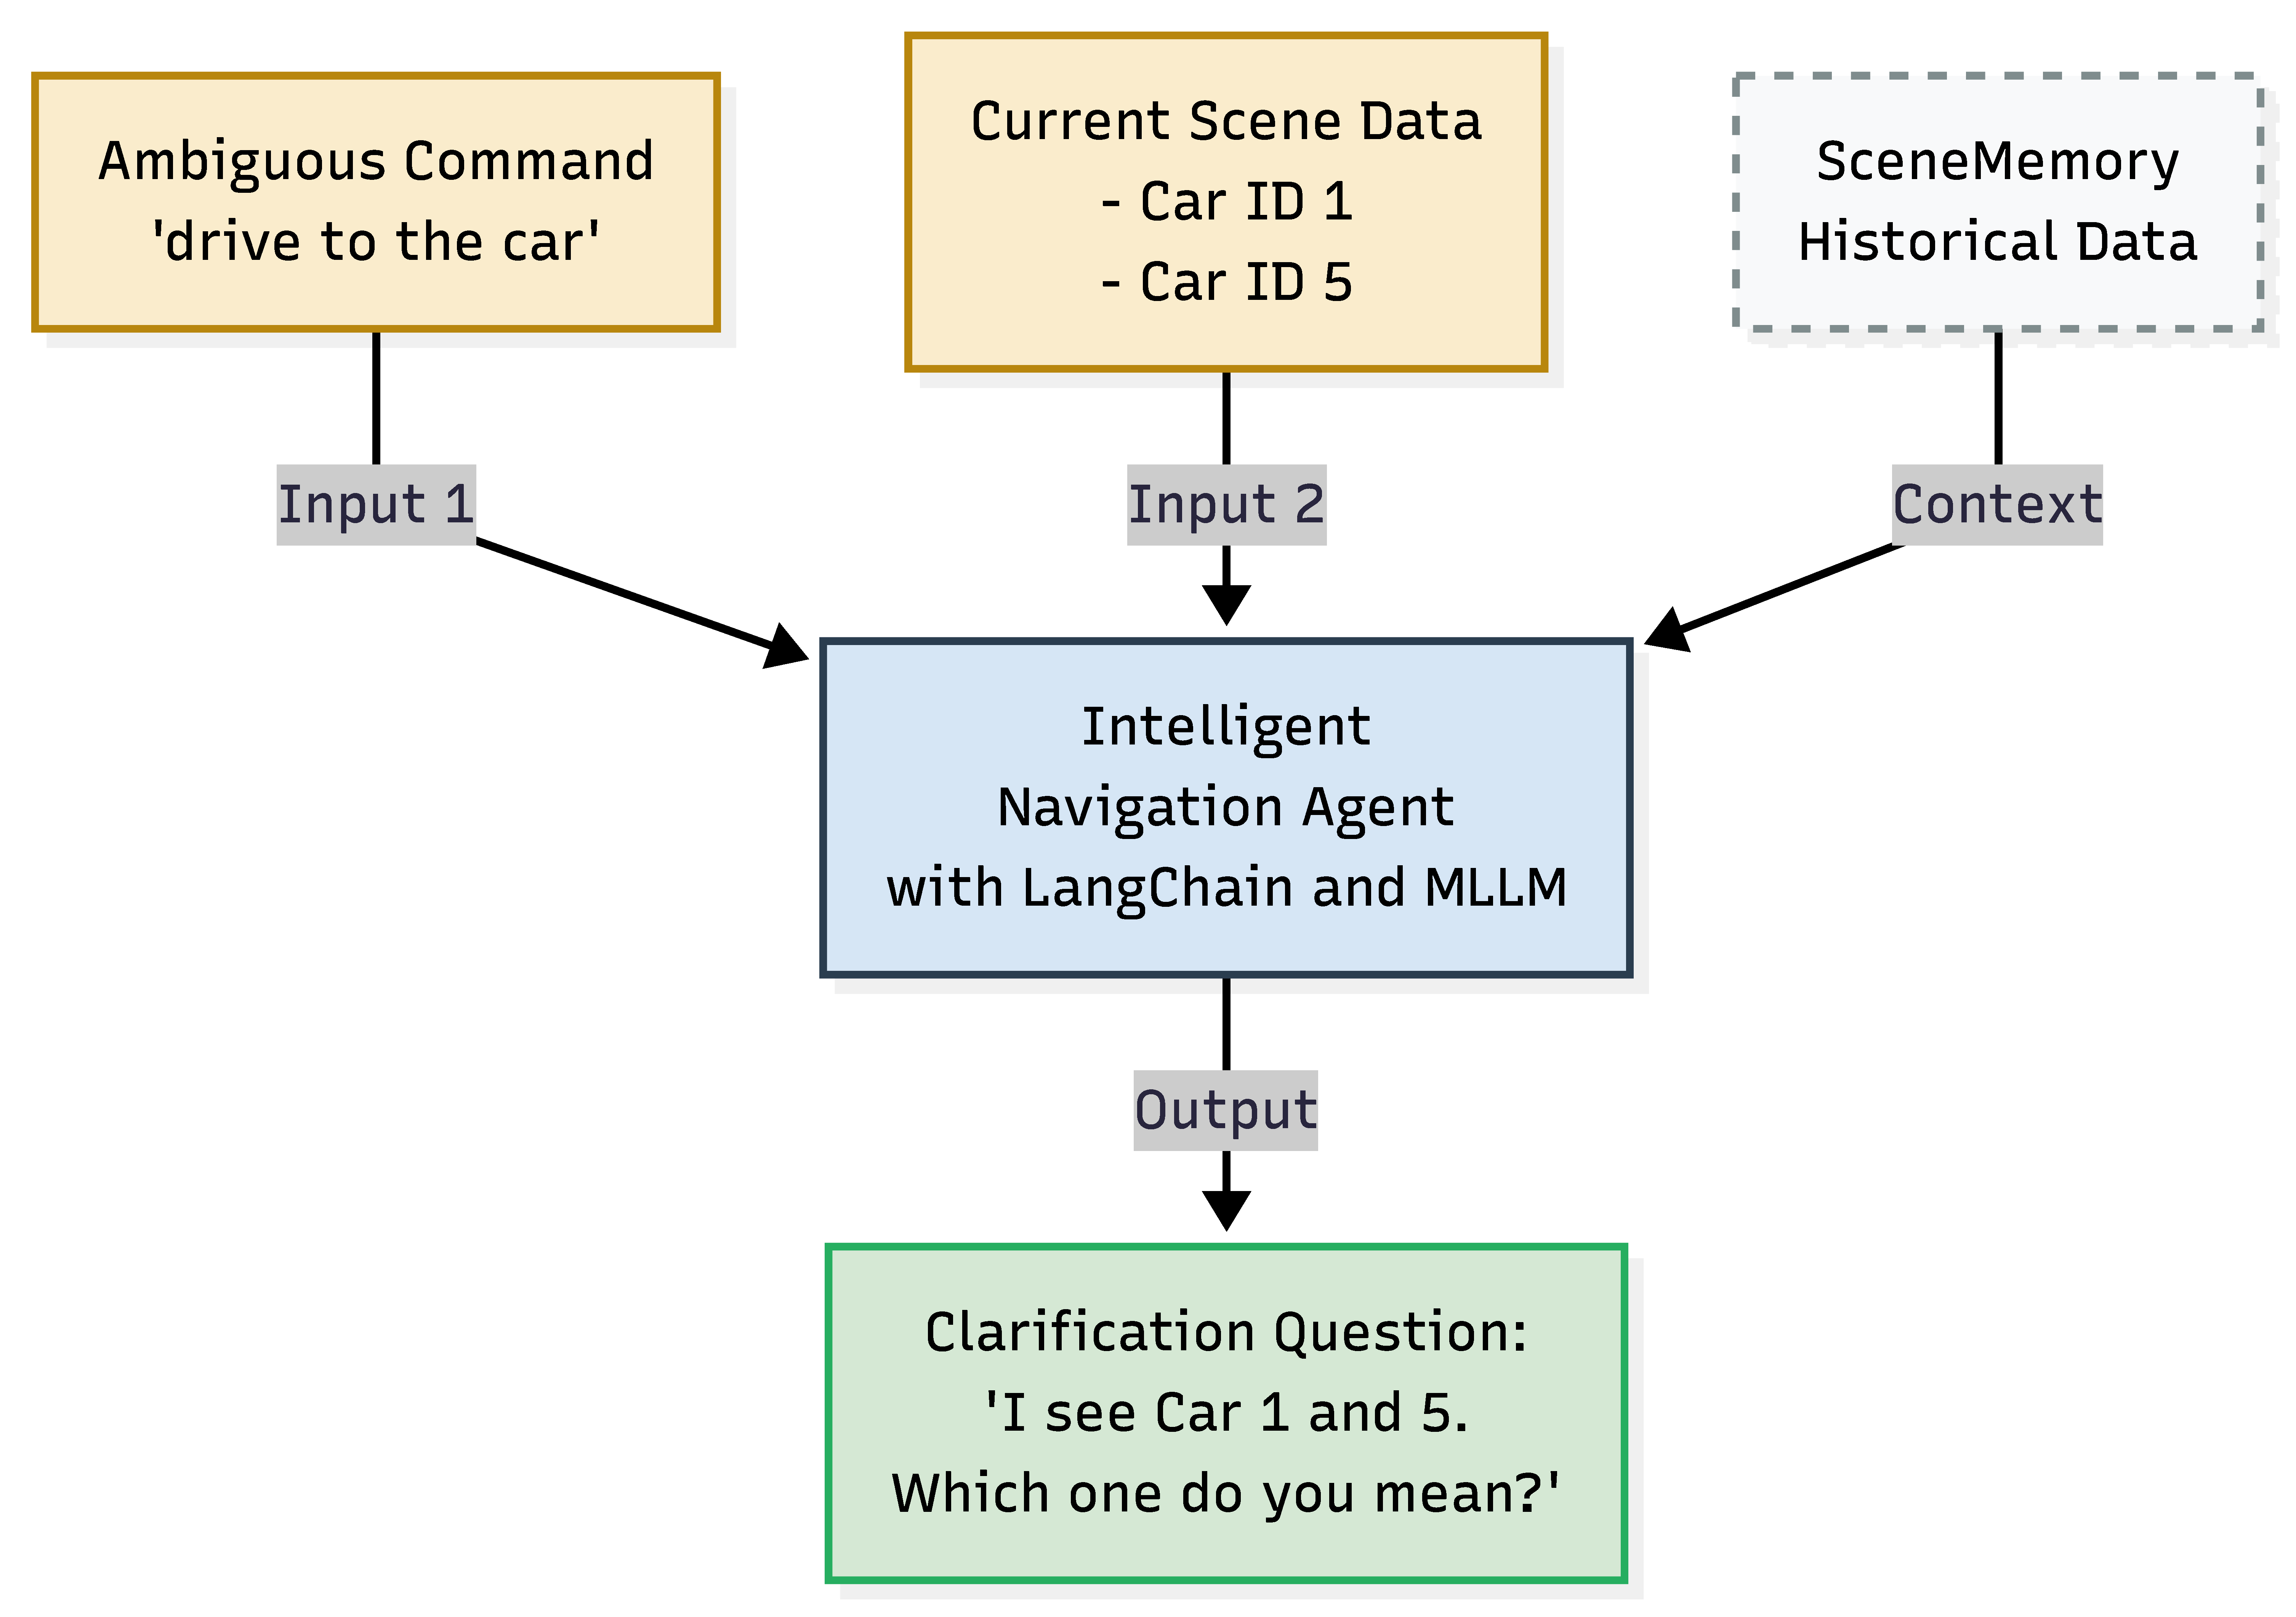
\includegraphics[width=\columnwidth]{./images/scenememory.pdf}
	\caption{The intelligent navigation agent is triggered in cases of ambiguity. It analyzes the current scene and uses historical data as context to generate a clarifying query for navigation via LangChain \cite{langchain}.}
	\label{scenememory}
\end{figure}


\section{Evaluation and Results}
\label{sec:experiments}

This section presents hardware test results and benchmarks obtained using YOLO models integrated into \textit{pAIrSEEption}, as well as the inference times of MLLMs such as Gemma~3 and Qwen~2.5~VL for generating scene descriptions. The second experiment reports results from two usability evaluations focusing on human-robot interaction and object-following tasks.

\subsection{Performance of YOLO-based Perception}

The average frames per second (FPS) and GPU utilization for several YOLO models of different sizes integrated into \textit{pAIrSEEption} are shown in Fig.~\ref{fig:yolo_comparison}. FPS is a key metric for evaluating the perception module because it directly affects system responsiveness, navigation accuracy, tracking performance, and overall operational safety.
The framework supports YOLO models in PyTorch (\textit{.pt}), \textit{.onnx}, and TensorRT (\textit{.engine}) formats. The TensorRT-optimized models (16-bit floating point) were evaluated on a laptop equipped with an Nvidia RTX A2000 GPU (8\,GB VRAM), 32\,GB RAM, and an Intel i7-13800H processor. The results demonstrate that the framework achieves strong performance even on consumer-grade hardware.
A confidence threshold of 40\% was set in the GUI during the experiments. Data were collected in a laboratory environment over 1750 frames containing both static and moving objects (moving objects were considered active). Performance metrics were recorded directly through the GUI and later used to generate the evaluation plots.
The results indicate that the \textit{yolo11n} (nano) model achieves the highest average FPS (just under 40 FPS), which is expected due to its small model size. The larger \textit{yolo11l\_TensorRT} model achieves comparable performance, demonstrating that TensorRT optimization improves throughput by approximately 5 FPS compared with the standard \textit{yolo11l.pt} model. 
Comparing the optimized TensorRT models, YOLOv11 outperforms YOLOv8 by roughly 5 FPS while increasing GPU utilization by only 2–3\%. As expected, segmentation models (indicated by the suffix \textit{seg} in Fig.~\ref{fig:yolo_comparison}) generally achieve lower FPS than their object-detection counterparts. However, segmentation masks could be beneficial for more precise obstacle avoidance in future work.


\begin{figure*}[!ht]
	\centering
	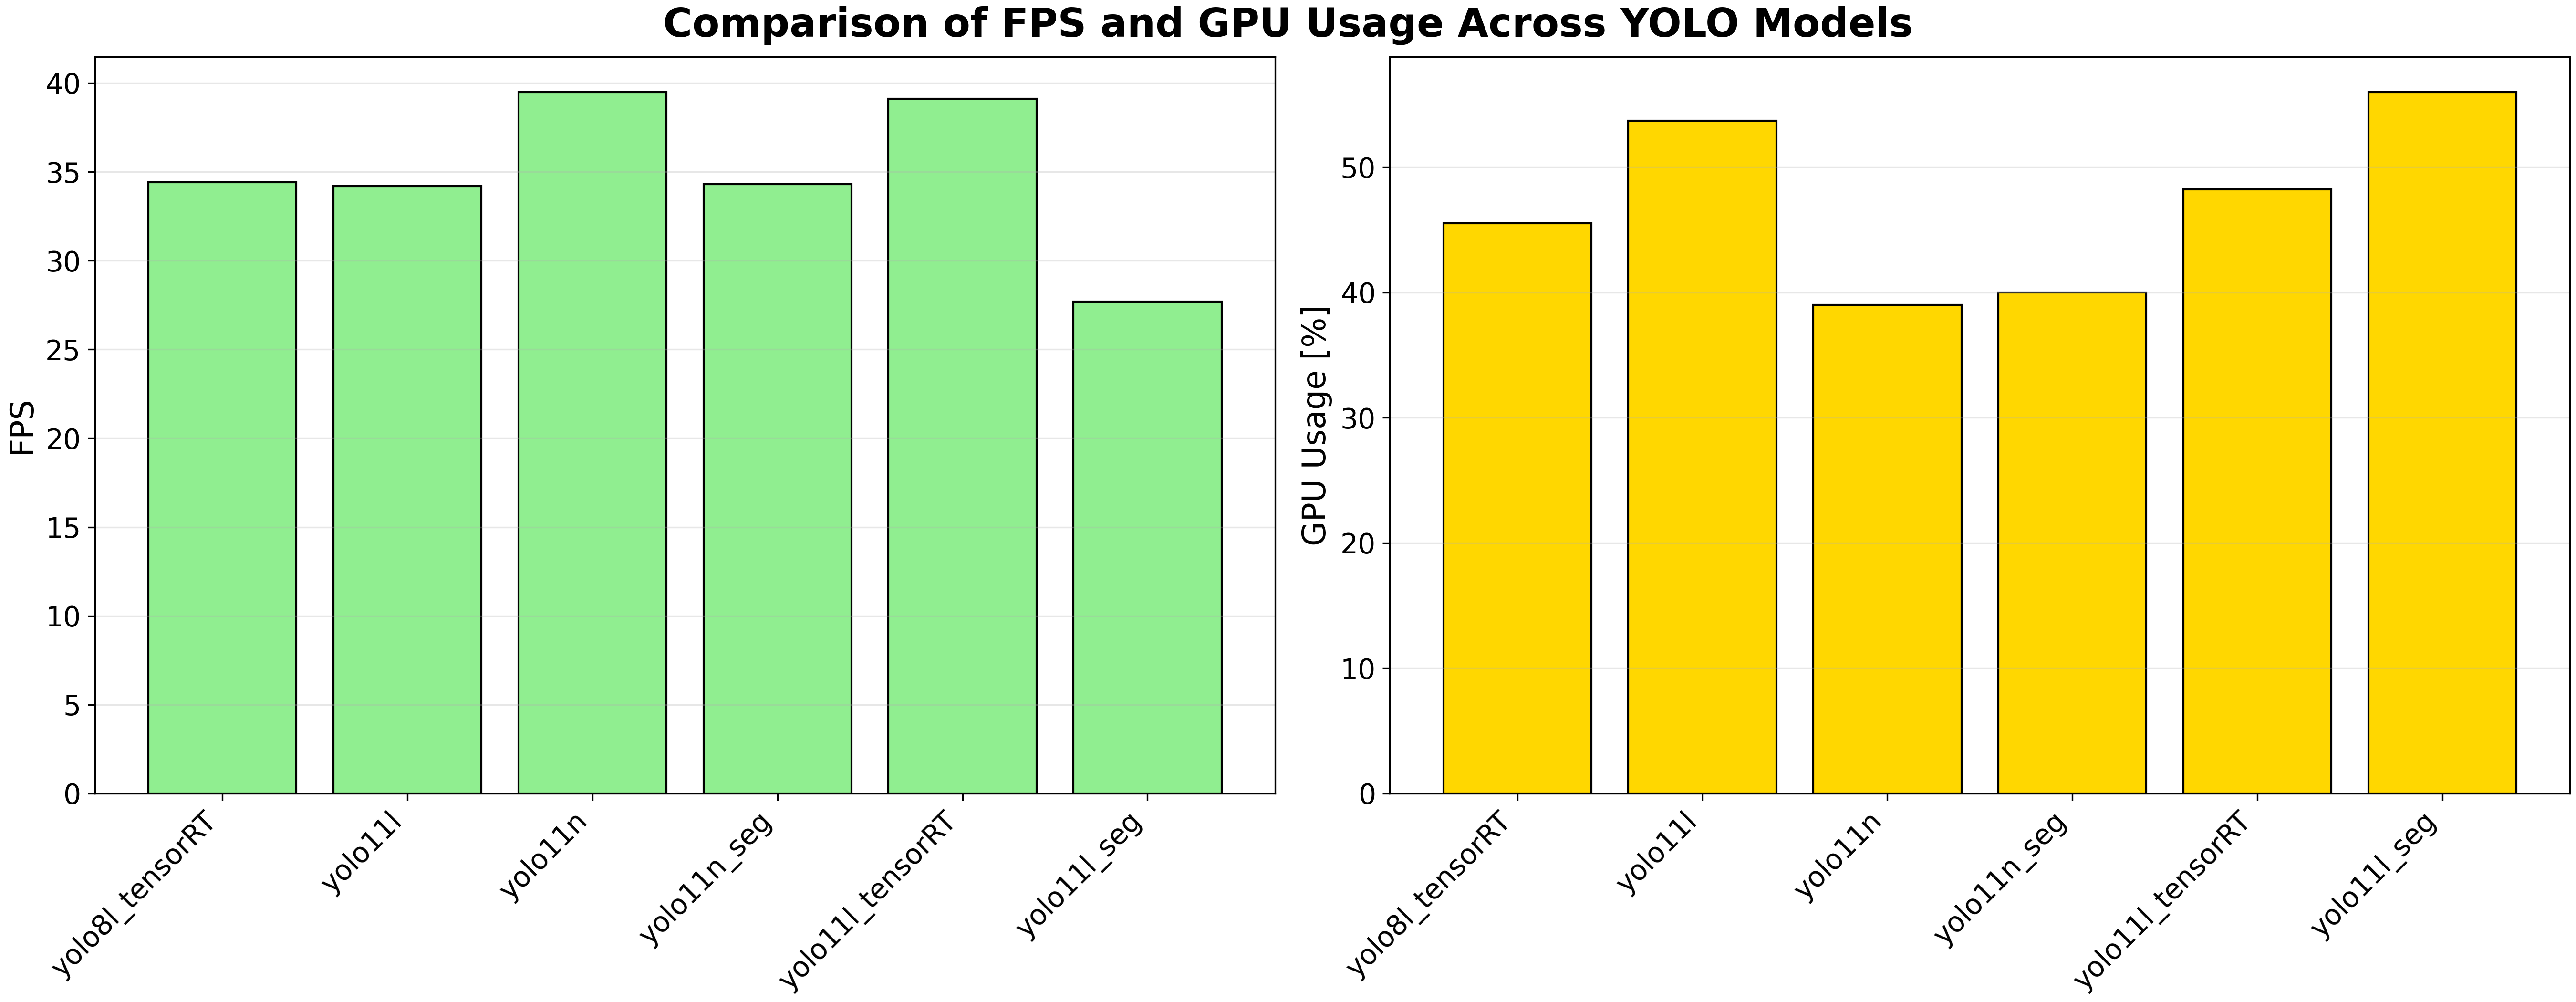
\includegraphics[width=\textwidth]{images/yolo_comparison.png}
	\caption{FPS and GPU usage analysis of YOLO models on the laptop with an average of 5.5 static and 1.1 active objects (objects in motion) captured over 1750 frames.}
	\label{fig:yolo_comparison}
\end{figure*}

\begin{figure}[!t]
	\centering
	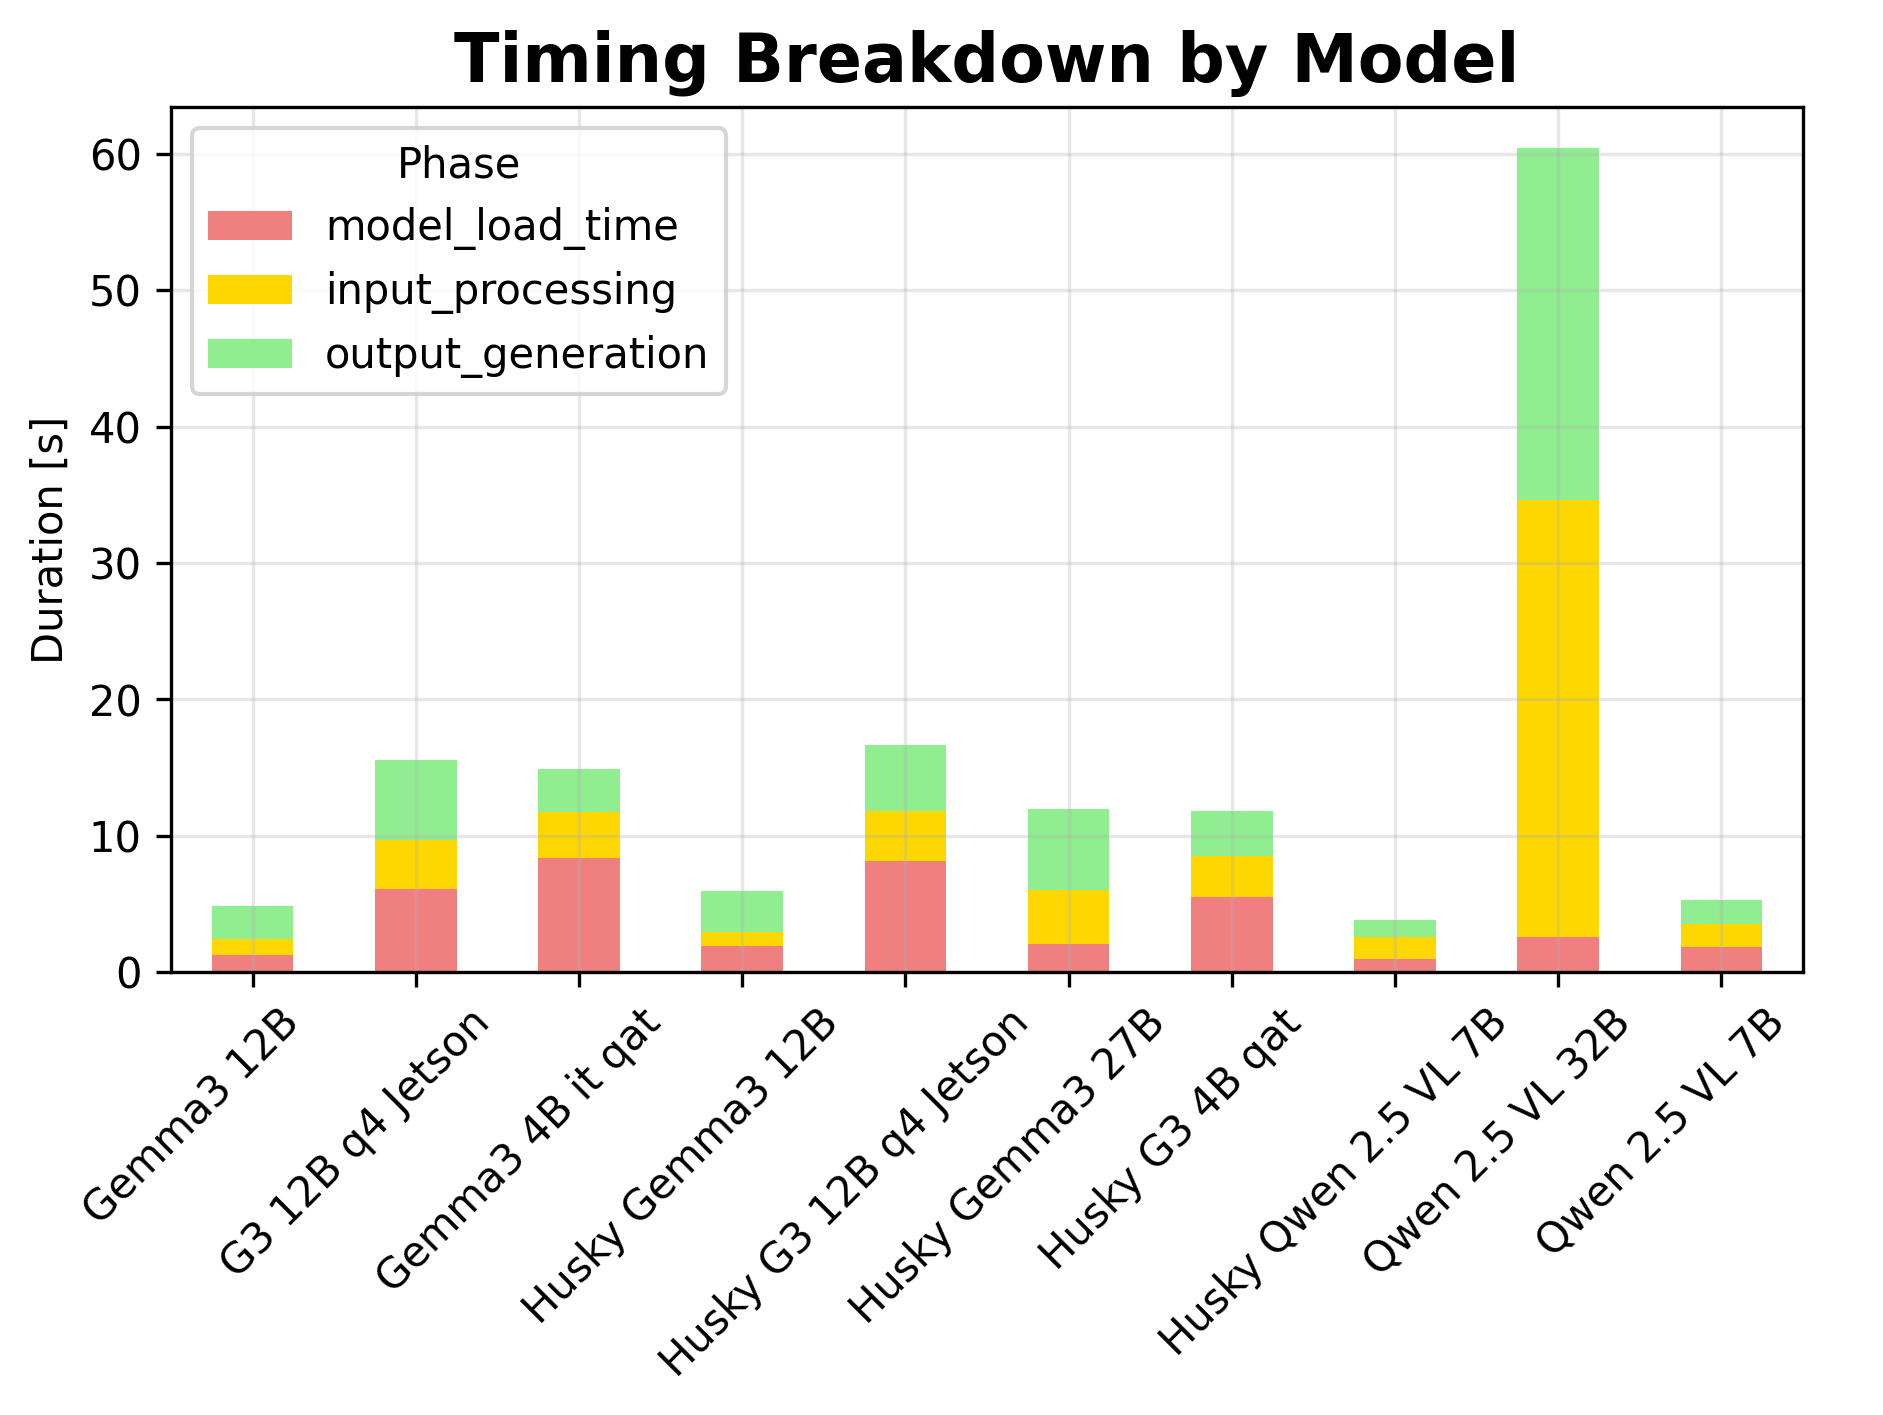
\includegraphics[width=8.5cm]{images/timing_breakdown.png}
	\caption{Timing breakdown of Gemma 3 and Qwen 2.5 VL models based on size. The suffix "Husky" indicates that the model has been modified using modelfile parameters and adapted to our application. Abbreviations: "G3" = Gemma 3, "it qat" = instruction-tuned and Quantization-Aware Training, "q4" = 4-Bit quantization.}
	\label{timing_breakdown}
\end{figure}

\begin{figure}[!htbp]
	\centering
	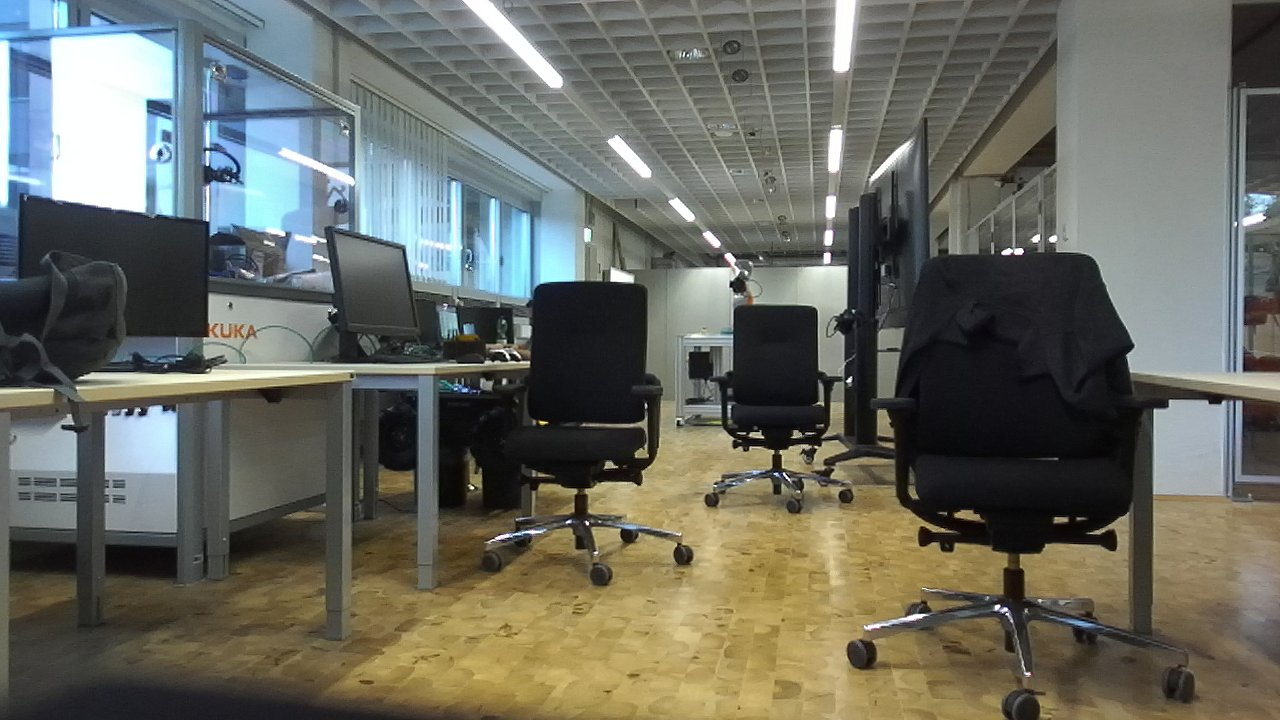
\includegraphics[width=\columnwidth] {images/lab.jpg}
	\caption{Qualitative assessment of Gemma 3 12B scene description capability. The model integrates real-time object detection data to generate a natural language representation of the robot's environment for assistive navigation. The scene description generated by a Gemma 3 12B model with spatial object data, reads as follows: \textit{"You are in a room, presumably an
			office. Directly in front of you,
			about 1.8 meters away and slightly to
			the left, is a screen. To your right,
			about 2.5 meters away, is a chair. To
			your left, about 3.7 meters away, is
			another chair. A little further ahead,
			about 4 meters away and to your left,
			is another screen. To your right,
			about 5 meters away, is another chair.
			Be aware of the chairs and screens as
			potential obstacles. The floor appears
			to be level."} This response was originally generated in German.}
	\label{mllm_scene_lab}
\end{figure}




\subsection{Performance of MLLM-Based  Scene Understanding}
\label{subsec:sceneunderstanding}



Fig.~\ref{timing_breakdown} presents the inference time of several Gemma~3 and Qwen~2.5~VL models for generating scene descriptions from object data. The measurements were recorded using Ollama logs, which contain metadata such as timestamps, unique identifiers (linking images and audio files to analysis logs), the model used for scene interpretation, and the number of input and output tokens. In all experiments, the same scene was evaluated across different models. The total response time, from the user request to the generated scene description, was divided into three components: model loading time, input processing time, and output generation time transmitted from the server to the client device running \textit{pAIrSEEption}. The runtime analysis shows that model size is the primary factor influencing system responsiveness. Very large models such as Qwen~2.5~VL~32B require more than 60~seconds to process a request and are therefore unsuitable for assistive applications given the server hardware constraints (Intel i9-13900KF CPU, RTX~A5000 GPU, and 128\,GB RAM). Smaller models such as Husky Qwen~2.5~VL~7B and Gemma~3~12B produce responses in under 6~seconds, making them suitable for near real-time operation. When running directly on the Jetson AGX Orin (32GB) platform (e.g., G3~12B~Q4 Jetson), the initial model loading time (\textit{model\_load\_time}) becomes the main latency bottleneck. The results also show that application-specific Husky customizations implemented via modelfiles introduce no measurable performance overhead. In practice, lightweight models with 7B or 12B parameters provide the best balance between performance and responsiveness. On Jetson systems, keeping the model resident in memory can further reduce loading delays. Fig.~\ref{mllm_scene_lab} illustrates a laboratory scene described by the Gemma~3~12B model. The generated output demonstrates strong spatial awareness and semantic coherence. By combining YOLO-based detections with ZED-derived depth information, the model effectively translates metric coordinates into natural language descriptions. The obstacles are ordered chronologically by distance (1.8\,m to 5.0\,m) without explicit instruction. Detected static objects are correctly identified as potential obstacles, indicating effective reasoning within the task-related layer of the SG. Additionally, the model remarks on global scene properties such as the floor condition,  stores and recalls last known attributes (e.g., identity, location, and task relevance) of objects  after occlusion/re-entrance (see Fig.~\ref{renentrance}), demonstrating persistent interpretation  beyond  YOLO preprocessing stages. This behavior supports a human-centered design that prioritizes user safety and situational awareness. Though focusing on locally hosted models,  experiments were also conducted with larger cloud-based MLLMs via OpenRouter (e.g., Llama~4~Scout/Maverick and Gemini~2), which produced similarly accurate scene descriptions.


\begin{figure}[ht]
	\centering
	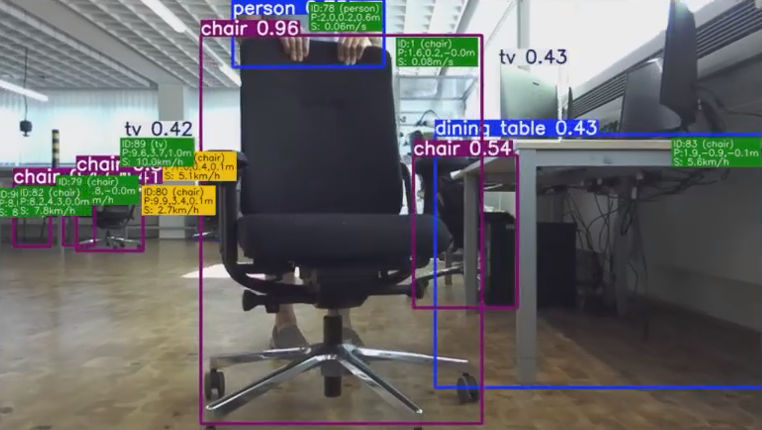
\includegraphics[width=\columnwidth]{pic/mental.png}
	\caption{\textit{Indoor} scene from the viewpoint of the robot mounted camera. Semantic perception of objects for structured description of the {indoor} environment by the mobile robot as SG-based mental model. The robot reasons over this graph using  MLLM and makes the decision to track the moving chair in response to the verbal human instruction and persistent context.}
	\label{mental1}
\end{figure}


\subsection{Target Attainment under Ambiguity}
\label{target_attainment_ambiguity}

This experiment evaluates whether the proposed task-grounding mechanism can prevent underspecified voice commands from being executed on the wrong target. The robot is verbally instructed to navigate to a chair. Two scenarios are considered. In the non-ambiguous case, only one chair is visible in the camera field of view (FOV). In the ambiguous case, multiple chairs are visible, as shown in Fig.~\ref{mllm_scene_lab}, and one is carried by a human, as shown in Fig.~\ref{chairhuman}. Each scenario is repeated ten times.

\begin{figure}[hb]
	\centering
	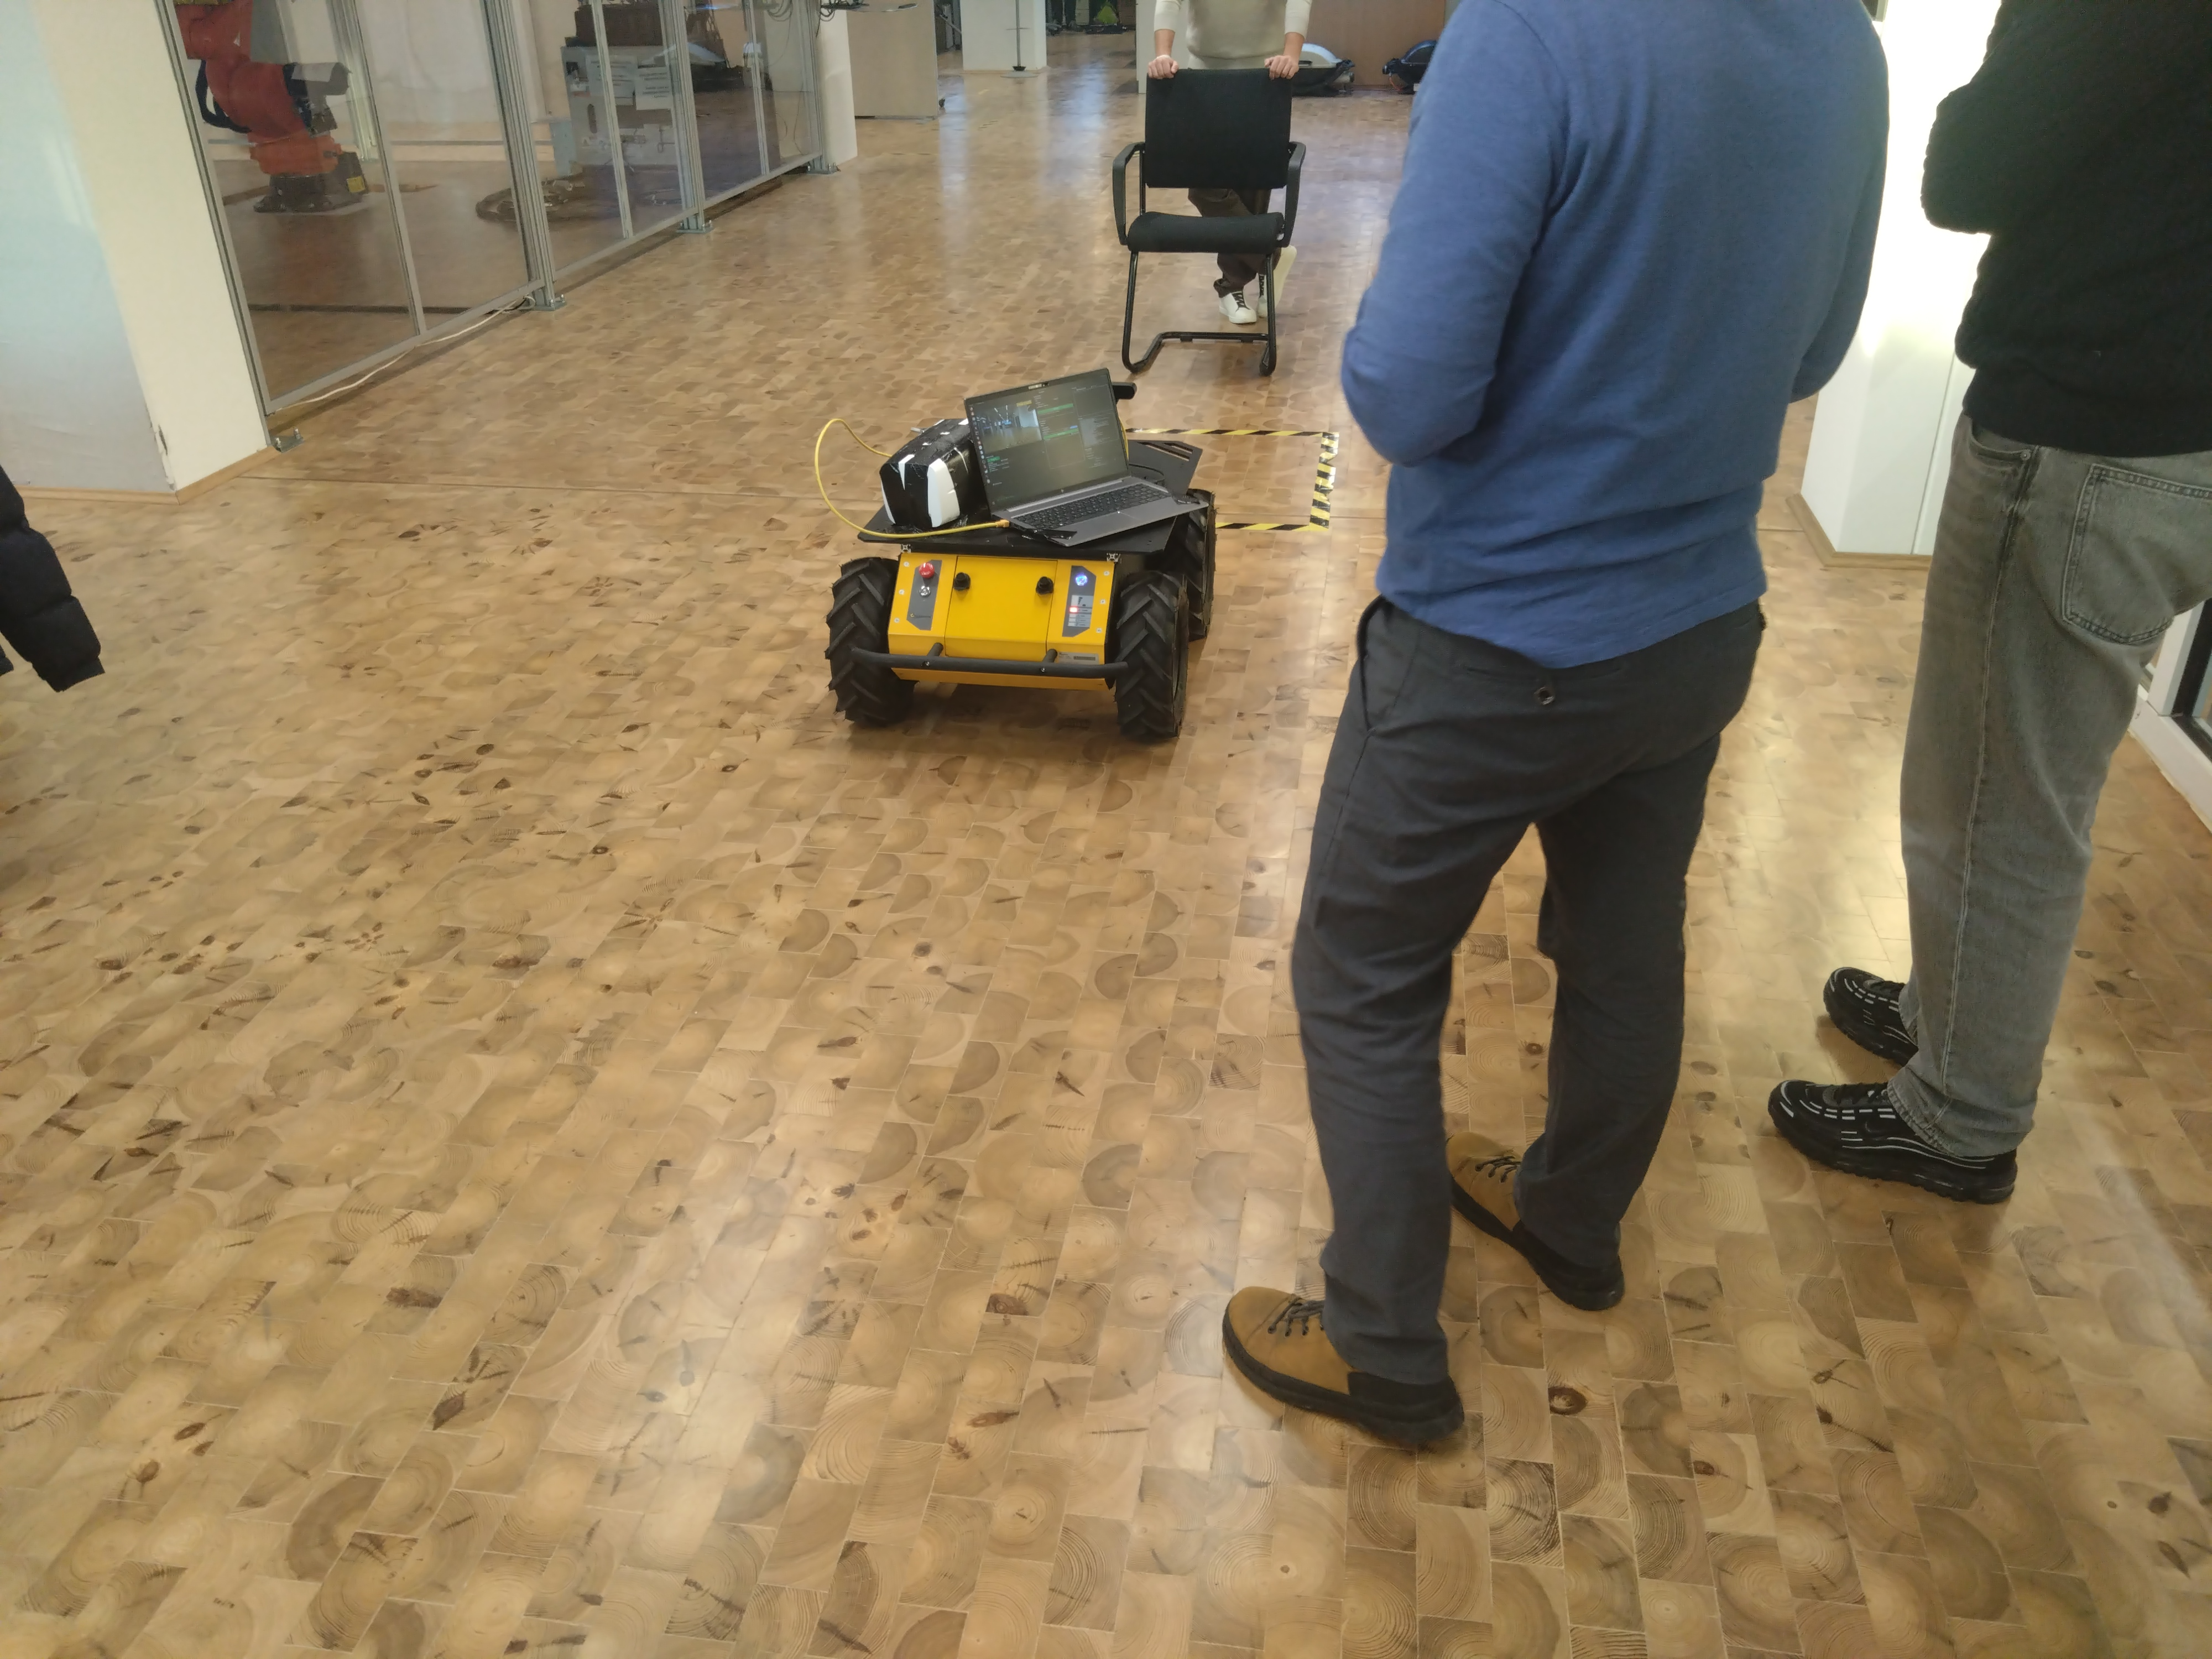
\includegraphics[width=0.98\columnwidth]{images/chairandhuman.jpg}
	\caption{Chair carried by a human.}
	\label{chairhuman}
\end{figure}

In all trials, the target objects and the human remain within the camera FOV. If the voice command cannot be reliably transcribed or parsed, for example because of background noise or poor audio quality, the robot does not execute the command immediately. Instead, it asks the operator to repeat or clarify the command. In the non-ambiguous case with a single visible chair, the system achieved a 100\% success rate for target-approach tasks.

The ambiguous case evaluates whether task grounding can prevent the robot from selecting an unintended chair when several candidate objects satisfy the same semantic class. After the user command is mapped to the semantic class \textit{chair}, the system retrieves the matching chair nodes from the current task-grounded SG. The candidate objects are then compared using their identifiers, spatial relations to the robot and user, visibility state, and semantic attributes derived from the current scene. If this comparison does not yield a unique target, the command remains underspecified. The system therefore formulates an explicit clarification question, for example: ``I see chair 1 on the left and chair 2 farther ahead, carried by a person. Which one do you mean?''

The operator resolves the ambiguity by specifying distinguishing properties through voice input or the graphical interface, such as the object identifier, spatial relation, or association with the human. The response is then mapped back to the corresponding SG node. This allows the robot to continue with a grounded command instead of executing an underspecified action. The experiment therefore tests the transition from task-grounded shared autonomy to supervised clarification under object-reference ambiguity. The success rate was 100\%.

\subsection{Memory-Enabled Autonomous Subgoal Selection}
\label{memory_enabled_subgoal_selection}

This experiment evaluates whether memory augmentation enables autonomous intermediate navigation decisions under intermittent perception. The operator provides only a final task command, such as ``navigate to the chair''. The robot must then determine whether a direct target approach is possible or whether an intermediate navigation reference is required. In contrast to the ambiguity experiment, the goal is not to ask the user which object is meant, but to test whether the robot can use memory-augmented scene context to continue execution without additional operator specification.

The test scene contains a chair that is initially observed in association with a person, for example because the person carries or temporarily occludes the chair. During the trial, the chair may become partially occluded or leave the camera field of view for a short time, as can be seen in Fig.~\ref{renentrance}. The memory-augmented SG stores the chair-person association, the last reliable chair position, the motion state of the associated person, and the confidence history of the object observations. When the chair is not directly available in the current frame, the robot selects an intermediate navigation reference from this memory context, such as the last reliable chair position or the current position of the associated person. This intermediate decision is generated autonomously and does not require an additional user command.

The experiment is repeated ten times. A trial is considered successful if the robot reaches the intended chair without switching to an unrelated object and without requiring the operator to specify an intermediate waypoint. The evaluation focuses on three aspects: recovery after temporary occlusion, stable object following after short perception dropouts, and reduced need for repeated user commands. These criteria assess whether memory augmentation provides temporal continuity, target persistence, and lower human intervention during autonomous task execution. A success rate of .. \%, .. \% and .. \% was yield for temporal continuity, target persistence, and lower human intervention during autonomous task execution.

To evaluate memory-augmented task grounding, we use four KPIs: task success (SR), temporal continuity (TCR), target persistence (TPR), and human intervention (HIR) rate. Task success measures whether the robot reaches the intended target. Temporal continuity quantifies whether the target remains associated with the same SG node across consecutive observations. For instance, the chair is detected in frame $t_0$, $t_0+\Delta t$, $t_0+2\Delta t$, but the bounding box jitters or confidence varies. Temporal continuity is high if the chair remains linked to the same SG node, e.g., chair\_2 (see Fig.~\ref{renentrance}), instead of switching between chair\_2, chair\_4, and chair\_1. Target persistence measures whether a temporarily lost target is correctly re-associated after occlusion or confidence loss. For example, the chair is visible as chair 3, then disappears behind a person for three seconds, then reappears. Target persistence is high if the system re-associates the reappearing chair with the original SG node chair 3. Human intervention captures clarification requests, repeated commands, and manual corrections per trial.

\begin{equation}
	\mathrm{SR} =
	\frac{N_{\mathrm{success}}}{N_{\mathrm{trials}}}
	\cdot 100\% ,
	\label{eq:success_rate}
\end{equation}

\begin{equation}
	\mathrm{TCR} =
	\frac{N_{\mathrm{same\_node}}}{N_{\mathrm{valid\_frames}}}
	\cdot 100\% ,
	\label{eq:temporal_continuity_rate}
\end{equation}

\begin{equation}
	\mathrm{TPR} =
	\frac{N_{\mathrm{reassociated}}}{N_{\mathrm{dropouts}}}
	\cdot 100\% ,
	\label{eq:target_persistence_rate}
\end{equation}

\begin{equation}
	\mathrm{HIR} =
	\frac{N_{\mathrm{clarifications}} + N_{\mathrm{repetitions}} + N_{\mathrm{manual\_corrections}}}
	{N_{\mathrm{trials}}}.
	\label{eq:human_intervention_rate}
\end{equation}

Their value after 10 trials as summarized in Fig.~\ref{tab:kpisr}.
\begin{table}[h]
	\centering
	\caption{Example table with five columns and two rows}
	\label{tab:kpisr}
	\begin{tabular}{|c | c|c|c|c|}
		\hline 
		KPI  $\slash$Value (\%) & SR  & TCR & TPR & HIR \\\hline
		\hline
		- & 100 & 100 & 75 & 10 \\
		%Value 6 & Value 7 & Value 8 & Value 9 & Value 10 \\
		\hline
	\end{tabular}
\end{table}
KPI values indicate that the robot  keeps the same SG node during normal tracking, but sometimes fails after occlusion or re-entry. \textcolor{green}{Reasons include the strict time constraints and spatial dependencies of the implemented tracking architecture. The memory-based scene graph uses a fixed temporal hysteresis (set to 1.5 seconds). If an occlusion exceeds this duration, the object is intentionally removed from short-term memory to avoid ghosting. This results in a new ID assignment when the object re-enters the scene. Ghosting is the tracking system’s incorrect tracking of an object even though it has already permanently disappeared from the scene. This artifact typically appears when kinematic state estimators continue to extrapolate an object's trajectory without receiving new sensory validation. The framework relies on the assignment of kinematic data based on predicted 3D trajectories (e.g., Kalman filtering) rather than on visual appearances (classical Re-ID). Since external semantic bounding boxes are fed into the tracking SDK, the system lacks visual capabilities for long-term recognition. Consequently, if a tracked object moves significantly during a perception failure, its reappearance deviates too greatly from the predicted spatial trajectory, resulting in a persistence error. A brief perception failure can be caused, for example, by FPS drops or loose wired connection. 
The anti-ghosting mechanism actively monitors a moving average of the detection probabilities. Significant fluctuations in the detection probability during partial occlusion trigger a safety adjustment if the value falls below a critical threshold (such as $30\%$). Although this has an unintended effect on target tracking during complex re-entries, it successfully prevents false alarms during target tracking and ensures navigational safety.}

% kalman filtering (as state estimator) according to forum posts for pseudo/alternative "Re-ID": 
% 1. https://community.stereolabs.com/t/object-detection-position-irregularities/6520
% 2. https://community.stereolabs.com/t/body-velocity-is-delayed/7845/4


This experiment demonstrates a higher level of autonomy than task-grounded target selection alone. Task grounding defines the intended goal, whereas memory augmentation provides the temporal context needed to bridge perception gaps and derive intermediate execution steps. The robot can therefore move along the autonomy continuum toward locally autonomous subtask execution, while the human remains involved only at the level of task specification.

\subsection{Usability Studies}
We conducted a total of two usability studies:
In the first phase, we conducted a usability study with a group of end users of the implemented framework, who tested the robot system on-site in a practical setting. To complement this, we also included a video-based assessment of recorded interactions with participants from or based in Africa, Asia and Europe in the second phase. Because of geographical distance and limited remote access, hands-on testing was not feasible for these participants. However, their input allowed us to capture perspectives shaped by different cultural contexts and local needs. While not equivalent to direct interaction with the  system, the video-based approach revealed additional insight into how the system is perceived across contexts.
%The following section first presents and analyzes the on-site field study. The design and analysis of the second video-based study follows thereafter.

\subsubsection{Phase 1: On-site Setup Expert Evaluation}

For the on-site testing, nine participants  with  engineering backgrounds (undergraduate and graduate students, two females and seven males) interacted with the Husky mobile robot indoors (see Fig.~\ref{mental1}) and outdoors (see Fig.~\ref{mental2}) using German voice commands (e.g., ``Folge Stuhl'' = ``Follow chair'', ``Folge Person~1'' = ``Follow person~1''). After a brief introduction to the GUI and system functionality, participants verbally instructed the robot to follow selected targets over distances chosen by themselves. Voice commands could also be used to stop navigation or switch to a different target. During operation, the robot provided audio feedback describing its objectives, state, and actions. After completing the interaction, participants anonymously evaluated their experience through a survey.
To evaluate the usability of the system, particularly voice control and object tracking (following a target with the mobile robot), a survey was conducted consisting of nine Likert-scale items (rated from 1 to 5) and three open-ended questions. The items were structured as follows:

\begin{itemize}[leftmargin=*]
	\item \textbf{Voice Control:} 
	\begin{enumerate}[label=Q\arabic*:, series=survey, widest=Q12, leftmargin=*]
		\item Ease of issuing instructions.
		\item Reliability of command recognition  and execution despite evolving tasks.
		\item Necessity of repetitions (negative item*). 
	\end{enumerate}
	
	\item \textbf{Context-Aware Object Tracking:} 
	\begin{enumerate}[label=Q\arabic*:, resume=survey, widest=Q12, leftmargin=*]
		\item Accuracy of object identification  in various contexts.
		\item System response time to navigation instructions. 
		\item Frequency of losing the target in evolving tasks (negative item*). 
	\end{enumerate}
	
	\item \textbf{User Experience:} 
	\begin{enumerate}[label=Q\arabic*:, resume=survey, widest=Q12, leftmargin=*]
		\item Overall ease of understanding and using the robot. 
		\item Perceived safety during operation. 
		\item Intention to use the system in real-world applications. 
	\end{enumerate}
	
	\item \textbf{Qualitative Feedback (Open-ended):} 
	\begin{enumerate}[label=Q\arabic*:, resume=survey, widest=Q12, leftmargin=*]
		\item Positive aspects of system operation. 
		\item Suggestions for improving user experience$\slash$comfort.
		\item Proposed additional functions or commands. 
	\end{enumerate}
\end{itemize}

\begin{figure}[ht]
	\centering
	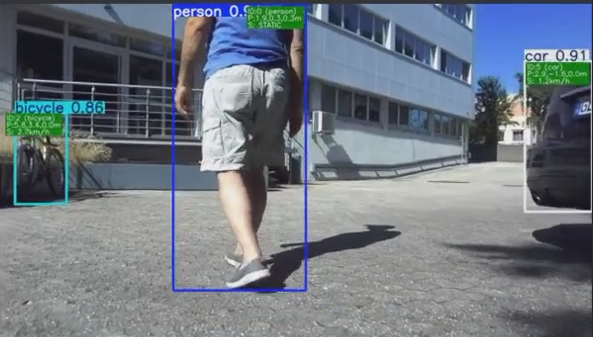
\includegraphics[width=\columnwidth]{pic/mental2.png}
	\caption{\textit{Outdoor} scene from the viewpoint of the robot mounted camera. The robot semantically understands the {outdoor} environment. It follows its human teammate {from behind} while providing real-time, natural-language insights into the usefulness of surrounding objects, facilitating smart mobility. These include obstacles (e.g., cars) and items relevant for active transportation (e.g., bicycles). By reasoning over relative pose, object affordances, and user needs, the robot with a \textit{task-grounded SG} assesses reachability and can guide its teammate toward cycling. This supports a vision of future society where robots seamlessly assist daily  activities and empower human self-determination.}
	\label{mental2}
\end{figure}


The questions $Q_{i,\, i \in \{1,\dots,9\}}$ were rated by participants (P1--P9) on a five-point scale, where 1 indicates the lowest/worst rating and 5 the highest/best rating. For questions Q3 and Q6 (negative items), responses were reverse-coded for statistical analysis (1 = best, 5 = worst). For each quantitative question (Q1--Q9), the mean $\bar{x}$ and the sample standard deviation (SD) $s$ were calculated. %Since participant P5 skipped question Q3, $n = 8$ was used to compute the mean and standard deviation for that item.

\subsubsection{Results and Discussion of Phase I}
\begin{table}[!b]
	\centering
	\caption{Quantitative Results of the Usability Evaluation ($N=9$) featuring Mean Score $\bar{x}$ and Sample Standard Deviation $s$. Scoring: 5 = highest/best, 1 = lowest/worst.
		*Negative questions: lower values indicate better performance.}
	\label{tab:user_study_results}
	\setlength{\tabcolsep}{3.5pt} 
	\begin{tabular}{|l|c|c|c|c|c|c|c|c|c|}
		\hline
		\textbf{Participant} & \textbf{Q1} & \textbf{Q2} & \textbf{Q3*} & \textbf{Q4} & \textbf{Q5} & \textbf{Q6*} & \textbf{Q7} & \textbf{Q8} & \textbf{Q9} \\ \hline
		P1 & 4 & 4 & 3 & 5 & 4 & 1 & 4 & 5 & 4 \\ \hline
		P2 & 4 & 4 & 3 & 5 & 5 & 1 & 4 & 5 & 4 \\ \hline
		P3 & 5 & 5 & 1 & 4 & 5 & 2 & 5 & 5 & 5 \\ \hline
		P4 & 5 & 5 & 1 & 5 & 5 & 2 & 5 & 5 & 5 \\ \hline
		P5 & 5 & 5 & $-$ & 4 & 5 & 1 & 5 & 5 & 5 \\ \hline
		P6 & 5 & 5 & 1 & 5 & 5 & 1 & 4 & 4 & 5 \\ \hline
		P7 & 5 & 4 & 2 & 5 & 4 & 3 & 4 & 4 & 3 \\ \hline
		P8 & 4 & 5 & 1 & 5 & 4 & 1 & 5 & 5 & 2 \\ \hline
		P9 & 5 & 4 & 2 & 5 & 4 & 2 & 5 & 4 & 5 \\ \hline \hline
		\textbf{Mean} $\bar{x}$ & \textbf{4.67} & \textbf{4.56} & \textbf{1.75} & \textbf{4.78} & \textbf{4.56} & \textbf{1.56} & \textbf{4.56} & \textbf{4.67} & \textbf{4.22} \\ \hline
		\textbf{SD} $s$ & \textbf{0.50} & \textbf{0.53} & \textbf{0.89} & \textbf{0.44} & \textbf{0.53} & \textbf{0.73} & \textbf{0.53} & \textbf{0.50} & \textbf{1.09} \\ \hline
	\end{tabular}
	\vspace{1ex}
\end{table}

The quantitative results in Table~\ref{tab:user_study_results} indicate a high level of user satisfaction across all evaluated categories. In particular, the ease of issuing voice commands and the perceived safety during robot operation received high ratings ($\bar{x}_{Q1,Q8} = 4.67$, $s_{Q1,Q8} = 0.50$). The accuracy of object identification achieved the highest mean score ($\bar{x}_{Q4} = 4.78$) with the lowest standard deviation ($s_{Q4} = 0.44$), indicating both strong performance and high agreement among participants.

High ratings were also observed for command recognition reliability, system response time, and overall usability ($\bar{x}_{Q2,Q5,Q7} = 4.56$), suggesting that the tracking behavior was perceived as predictable and safe. Participants also expressed a strong willingness to use such a system in real-world applications ($\bar{x}_{Q9} = 4.22$). Conversely, the low scores for the necessity of command repetition ($\bar{x}_{Q3} = 1.75$) and the frequency of losing  tracked   previously unseen targets and task contexts ($\bar{x}_{Q6} = 1.56$) further indicate that both the voice control and object tracking performed higly reliable. The low standard deviations across items suggest a strong consensus among participants.

%\textcolor{blue}{Independent of the participant usability study, an end-to-end system test was conducted, where a $100\%$ success rate for target approach tasks was archived. In these tests, the robot was verbally commanded to navigate to specific objects (e.g., people or chairs) using their unique ID numbers. This test was repeated ten times. It showed that target selection was accurate even among identical object classes. The assessment focused strictly on approaching targets that remained within the camera's FOV without taking complex Re-ID processes into account. If the voice command is unclear (e.g., due to background noise, poor audio quality, etc.), the robot will ask for clarification, before performing any action.}

However, this study has several limitations. All participants had engineering backgrounds and were undergraduate or graduate students, reflecting a relatively high level of technical familiarity and intrinsic interest in robotics. As such, usability and acceptance are likely to differ for non-expert users, particularly in real-world societal contexts. Furthermore, the small sample size ($N=9$) limits generalization and positions this study as a pilot evaluation. Despite these limitations, the findings demonstrate the framework’s potential to enable context-aware, intuitive, and task-grounded human–robot interaction.

Future studies should involve visually impaired users to evaluate the practical usefulness of the generated scene descriptions (Fig.~\ref{mllm_scene_lab}) for independent navigation. Moreover, although object tracking performance was rated highly in the current controlled environment, future work should investigate more cluttered or unstructured settings where the probability of losing the target (Q6) may increase.

Qualitative feedback (Q10-Q12) revealed both strengths in operational performance and areas for improvement. The system’s precision, responsiveness, interface clarity, and stable distance maintenance during following tasks were consistently highlighted, while smoother turning behavior and broader language support were identified as key areas for enhancement. Although the current architecture employs faster-whisper for automatic language recognition (input), TTS output remains limited to German. Given the multilingual capabilities of the integrated MLLMs, extending language support is a key direction for future development.

\textcolor{red}{
Further recommendations included the integration of true visual object Re-Identification (Re-ID) networks to complement the current kinematic data association to improve the target persistence rate beyond the current 75\%. Additional suggestions were improvements in obstacle detection and voice command guidance, as well as additional functionalities such as reverse driving, 180$^\circ$ turning, robotic arm integration, and inter-robot communication. The need for fallback mechanisms to handle voice-signal loss and for additional communication modalities to enhance robustness was also highlighted. Overall, these findings indicate that the proposed system lowers the barrier to human-robot teaming and demonstrates strong potential for service robotics in societal environments.}

\subsubsection{Phase 2: Remote and Global  Video-based Study}
The second group comprised 10 additional participants without prior robotics experience, representing a broad demographic spectrum (ages 8–74 years, mean $\bar{x}_{age} = 43.9$, five male and five female) across Africa, Asia, and Europe. In this phase, participants evaluated the system based on two videos: one showing verbal human-robot interaction and demonstrating navigation and object-tracking capabilities in an indoor environment, and the other demonstrating human-following with assistance and guidance in an outdoor environment. The qualitative assessment was structured around three condensed questions, consistent with Phase I: interaction quality, trust in navigation and system behavior, and practical utility.

The results indicate a comparable level of perceived usefulness to that observed in Phase I. Nine participants described the interaction as natural, reflecting overall positive perceptions, while one participant did not respond. High levels of trust were reported in both navigation and conversational capabilities, with particularly strong confidence among younger European participants. However, two participants from Africa emphasized the need to improve technical reliability in dynamic or structurally challenging environments (e.g., complex road conditions or flooded areas).

These findings highlight the importance of evaluating SG-based semantic understanding under diverse environmental and seasonal conditions to further assess the robustness of the system’s reasoning and navigation. Participants also identified practical applications in logistics, agriculture, and retail. Notably, the system received high acceptance among  participants, particularly in the context of elderly care and daily assistance in African settings. Feedback from Africa and Asia further underscores the importance of supporting local languages to facilitate adoption, improve global accessibility and user experience. Overall, the second-phase study indicates a high potential for social acceptance, even among non-expert users.

\section{Conclusion}\label{conclusion}

This work introduced a framework for SGG that integrates precise 3D sensor data with the semantic reasoning capabilities of MLLMs for mobile robotics. By transforming structured metric object data into natural language representations, the proposed approach bridges perception and semantic understanding, enabling both human interpretability and actionable awareness of the environment. The resulting SGs support intuitive navigation, assistance, and guidance, making robotic behavior more transparent and accessible, particularly for users with limited visual perception. Experimental results demonstrate that grounding MLLM reasoning in sensor data leads to factually consistent scene interpretations, while user studies confirm high perceived reliability, safety, and social acceptance. Overall, this work advances toward extended, human-centered robot intelligence, in which robots can reason about their environment and communicate this understanding at a high level to support inclusive and meaningful human–robot collaboration. The proposed framework empowers users to better understand, guide, and collaborate with robotic systems in real-world environments, paving the way for a more inclusive and capable robotized society. Toward this vision, we move closer to robots that are task-grounded, memory-augmented, and capable of introspection. These robots can combine perception, task context, and interaction history to generate human-interpretable explanations of their environment and behavior.

\section*{Acknowledgments}
The authors would like to thank Mr. N. Mahr and Mr. N. Schenkel for their support in conducting the task grounding and memory augmentation study, and Mr. A. Koennecke for his support with robot control. The authors also thank all participants for their time and valuable feedback.

During the preparation of this manuscript, the author(s) used the GPT-5.3 model to improve the language and readability. After using this tool, the authors reviewed and edited the content as necessary. 
\bibliographystyle{IEEEtran}
\bibliography{references}


%\newpage





\vfill

\end{document}


